%------------------------------------------------------------------------------
%
%  Documentation "Data Logging Service"
%
%  Ingenieurgemeinschaft IgH
%
%  Author: Florian Pose
%
%  $Id$
%
%  vim: spelllang=en spell tw=78
%
%  Permission is granted to copy, distribute and/or modify this document under
%  the terms of the GNU Free Documentation License, Version 1.3 or any later
%  version published by the Free Software Foundation; with no Invariant
%  Sections, no Front-Cover Texts and no Back-Cover Texts. A copy of the
%  license is included in the file fdl-1.3.txt.
%
%------------------------------------------------------------------------------

\documentclass[a4paper,12pt,BCOR6mm,bibtotoc,idxtotoc]{scrbook}

%\usepackage[english]{babel}
\usepackage[french]{babel}
\usepackage[utf8]{inputenc}
\usepackage{graphicx}
\usepackage[automark,headsepline]{scrpage2}
\usepackage{makeidx}
\usepackage{listings}
\usepackage[nofancy]{rcsinfo}
\usepackage{hyperref}

\lstset{basicstyle=\ttfamily\small}
\lstset{numberstyle=\tiny}
\lstset{aboveskip=4mm}
\lstset{belowskip=2mm}
\lstset{escapechar=`}

\hypersetup{pdfpagelabels}
\hypersetup{plainpages=false}
\hypersetup{linkcolor=blue}
\hypersetup{urlcolor=blue}
\hypersetup{colorlinks=true}

\setlength{\parskip}{1.5ex plus 0.8ex minus 0.5ex} \setlength{\parindent}{0mm}

\newcommand{\IgH}{\raisebox{-0.7667ex}\
    {
\includegraphics[height=2.2ex]{bilder/ighsign}}}

\DeclareFontShape{OT1}{cmtt}{bx}{n} {
<5><6><7><8><9><10><10.95><12><14.4><17.28><20.74><24.88>cmttb10 }{}

\rcsInfo $RCSId$

\makeindex

\begin{document}

%------------------------------------------------------------------------------

% Titelseite

\pagenumbering{roman} \pagestyle{empty}

\begin{titlepage} \begin{center} \rule{\textwidth}{1.5mm}

{\Huge\bf Data Logging Service (DLS)\\[1ex] Version 1.2}

\vspace{1ex}

\rule{\textwidth}{1.5mm}

\vspace{\fill}

{\Large Florian Pose, \url{fp@igh-essen.com}\\[1ex]
    Ingenieurgemeinschaft \IgH}

\vspace{\fill}

``DLS'' est un syst\`eme d'archivage capable de collecter des
donn\'ees hautes fr\'equences pendant une longue p\'eriode et de les
stocker sous forme tr\`es compress\'ee.  Son objectif est d'offrir
\`a l'utilisateur un acc\`es performant et sans limite aux donn\'ees
enregistr\'ees, aussi bien la vue d'ensemble annuelle qu'une infime
fluctuation pendant une fraction de seconde.

\vspace{\fill}

{\large Essen, \rcsInfoLongDate\\[1ex] R\'evision \rcsInfoRevision}

{\large Traducteur: S\'ebastien BLANCHET}

\end{center}
\end{titlepage}

%------------------------------------------------------------------------------

% Inhaltsverzeichnis

\pagestyle{scrheadings}

\tableofcontents

%------------------------------------------------------------------------------

% Dokument

\chapter{G\'en\'eralit\'es}
\label{sec:allg}
\pagenumbering{arabic}

%------------------------------------------------------------------------------

\section{Principe de l'acquisition de donn\'ees}
\label{sec:allg_grund}

``Data Logging Service'' (ci-apr\`es \textit{DLS})\index{DLS} est un
syst\`eme d'enregistrement de donn\'ees qui est non seulement capable
de collecter, compresser et stocker tout type de mesures pendant une
longue p\'eriode, mais aussi de les afficher rapidement chaque fois que
n\'ecessaire.

Le pr\'erequis pour un processus d'acquisition de donn\'ees est une
\textit{source de donn\'ees}\index{datasource!Definition}, qui fournit
les donn\'ees mesur\'ees. Dans ce cas, il s'agit d'un serveur r\'eseau
qui fournit les donn\'ees mesurées via \textit{rt\_lib}, une
biblioth\`eque d\'evelop\'ee par \textit{IgH}.  La communication avec
la source de donn\'ees est d\'ecrite dans
\autoref{sec:dlsd_logger_comm}.

Toutes les donn\'ees \`a livrer sont organis\'ees en
\textit{canaux}\index{channel!definition}. Un canal est une abstration
d'une quantit\'e physique mesurable fournie par la source de
donn\'ees.  Les propri\'et\'es du canal sont
l'unit\'e\index{channel!unit}, la fr\'equence maximale
d'\'echantillonnage\index{channel!sampling frequency} et le type de
donn\'ee\index{channel!data type}.

DLS peut se connecter aux sources de donn\'ees puis interroger les
informations via les canaux fournis.  De la m\^eme mani\`ere, il est
alors capable de demander et de recevoir les donn\'ees pour des canaux
sp\'ecifiques.

%------------------------------------------------------------------------------

\section{T\^aches d'acquisition}
\label{sec:allg_jobs}

DLS enregistre les donn\'ees par l'interm\'ediaire de \textit{t\^aches
  d'acquisition}\index{measurement job!definition}.  Elles comprennent
les sp\'ecifications g\'en\'erales pour l'acquisition de donn\'ees
dont la liste des canaux \`a inclure et leurs sp\'ecifications.  Une
t\^ache d'aquisition est toujours li\'ee \`a une source particuli\`ere
de donn\'ees. Un nombre quelconque de t\^aches d'aquisition existent
simultan\'ement.

Une t\^ache d'acquisition peut recevoir simultan\'ement les donn\'ees
de diff\'erents canaux.  Cela n\'ecessite que chaque canal soit
\'etiquet\'e avec une \textit{sp\'ecification de canal}\index{channel
  specification} qui r\'ecaptitule les conditions de rappatriement et
de stockage des donn\'ees.  Ceci inclut la fr\'equence
d'\'echantillonnage, la taille des blocs, les m\'eta-donn\'ees \`a
r\'ecup\'erer (voir \autoref{sec:dlsd_data_meta}), le ratio de
m\'eta-r\'eduction et la m\'ethode de compression.

%------------------------------------------------------------------------------

\section{Stockage des donn\'ees}
\label{sec:allg_ablage}

Les donn\'ees captur\'ees sont stock\'ees dans le r\'epertoire de
donn\'ees de DLS\index{DLS data directory} conjointement avec les
sp\'ecifications de l'acquisition, le temps et les informations du
canal puis tri\'ees par t\^ache d'acquisition. Par d\'efaut, il s'agit
du r\'epertoire courant. Si un autre emplacement de stockage est
choisi, cette information peut \^etre communiqu\'ee aux programmes de
DLS soit via la ligne de commande (option \texttt{-d}), soit via la
variable d'environnement \$DLS\_DIR\index{\$DLS\_DIR}.  L'ordre de
pr\'evalence est toujours le suivant: ligne de commande -- variable
d'environnement -- r\'epertoire courant.

Plusieurs r\'epertoires de donn\'ees DLS peuvent coexister
simultan\'ement \`a condition qu'ils soient g\'er\'es par
diff\'erentes instances du daemon DLS (voir
\autoref{sec:dlsd_mother}).

Une description d\'etaill\'ee de la structure du r\'epertoire de
donn\'ees DLS et des donn\'ees qu'il contient, se trouve dans
\autoref{sec:data}.

%----------------------------------------------------------------------------

\section{Outils}
\label{sec:allg_tools}
\index{tools}

\begin{description}

\item[DLS Manager]\index{DLS Manager} Les t\^aches d'acquisition
  peuvent \^etre \'edit\'ees via l'interface graphique de \textit{DLS
    Manager} (voir \autoref{sec:manager}). Le programme permet de
  cr\'eer de nouvelles t\^aches et de modifier celles qui existent
  d\'ej\`a, m\^eme pendant les aquisitions.  L'utilisateur peut aussi
  visualiser la liste des t\^aches en cours d'ex\'ecution.

\item[DLS View] Un outil graphique \textit{DLS View}\index{DLS View}
  permet de visualiser les donn\'ees (voir
  \autoref{sec:view}). L'utilisateur peut afficher n'importe quel
  canal au-dessus d'une \'echelle de temps commune. Il est alors
  possible de naviguer dans la fen\^etre temporelle et de lire les
  valeurs individuelles.

\item[dls] L'outil en ligne de commande \textit{dls}\index{dls (tool)}
  permet de visualiser et d'exporter les donn\'ees d\'ej\`a enregistr\'ees.
  Voir \autoref{sec:apx_cmd_dls} pour la liste des sous-commandes.

\item[Script d'initialisation]\index{Init Script} Un script
  d'initialisation est fourni pour d\'emarrer et stopper dlsd et les
  services associ\'es.  Il reconna\^it les param\^etres
  \texttt{start}, \texttt{stop}, \texttt{restart} et
  \texttt{status}. La configuration du service est effectu\'ee via le
  fichier sysconfig\index{sysconfig file} qui contient toutes les
  variables n\'ecessaires.  Il est recommand\'e d'exporter les
  variables incluses via le script profile \'egalement fourni, pour
  les rendre ainsi accessibles \`a tous les utilisateurs.

\item[dls\_status] Le script \textit{dls\_\-status}\index{dls\_status}
  sert \`a la supervision g\'en\'erale des acquisitions. Cet un outil
  en ligne de commande peut afficher l'\'etat de sant\'e fondamental
  de l'acquisition pour un r\'epertoire de donn\'ees DLS sp\'ecifique.
  Il indique si le processus parent DLS est en cours d'ex\'ecution,
  quelles t\^aches d'acquisition sont disponibles et si les processus
  correspondants sont en cours de fonctionnement.

\end{description}

%------------------------------------------------------------------------------

\chapter{Le daemon DLS (dlsd)} \label{sec:dlsd}

Le \textit{daemon DLS} (en abr\'eg\'e: \textit{dlsd}) sert \`a
l'ensemble de l'acquisition et du stockage de
donn\'ees\index{dlsd}. C'est un processus qui tourne en t\^ache de
fond (sans \^etre connect\'e \`a la console) et qui li\'e \`a un
r\'epertoire sp\'ecifique de donn\'ees DLS\index{DLS data  directory}.
Il doit toujours \^etre en fonctionnement lors d'une
acquisistion.

\autoref{fig:arch} repr\'esente l'architecture\index{architecture} du syst\`eme.

\begin{figure}[htb]
  \begin{center}
    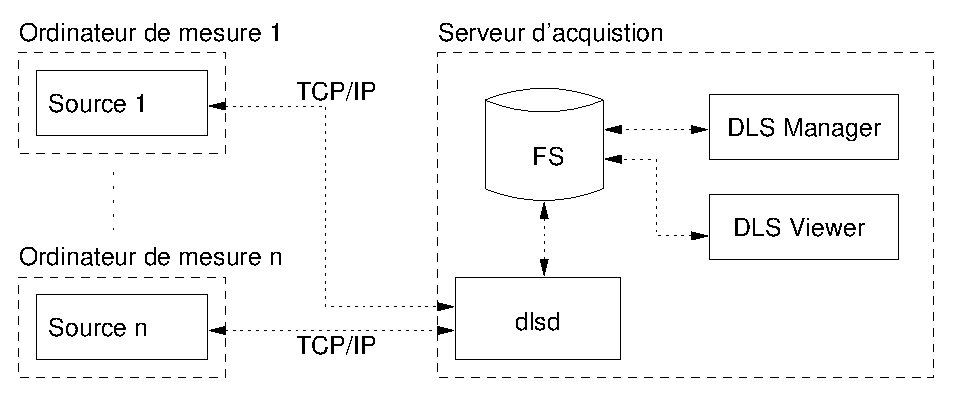
\includegraphics[width=350pt]{bilder/arch_fr}
  \end{center}
  \caption{Architecture}
  \label{fig:arch}
\end{figure}

%------------------------------------------------------------------------------

\section{Le processus parent dlsd}
\label{sec:dlsd_mother}
\index{dlsd!parent process}

La commande \texttt{dls start} d\'emarre un processus dlsd de
surveillance des t\^aches d'acquisitions\index{measurement job}. Il
est appel\'e le \textit{processus parent dlsd}.  Il contient une copie
des sp\'ecifications des t\^aches existantes dans le r\'epertoire de
donn\'ees DLS, ainsi que les informations des processus d'acquisition
associ\'es.

Chaque processus parent doit fonctionner dans un r\'epertoire de
donn\'ees DLS\index{DLS data directory} diff\'erent.  Ceci est garanti
par les m\'ecanismes de protection mis en oeuvre (\textit{fichiers
  PID}\index{PID files}, voir \autoref{sec:apx_pid}).

%------------------------------------------------------------------------------

\subsection{Comportement du processus parent dlsd}
\label{sec:dlsd_mother_behaviour}

Au d\'emarrage, le processus parent lit toutes les sp\'ecifications
des t\^aches d'acquisition dans le r\'epertoire de donn\'ees DLS et
cr\'ee un processus enfant pour chaque t\^ache d'acquisition active
\index{measurement job} (\textit{processus d'acquisition dlsd}, voir
\autoref{sec:dlsd_logger}), qui servira ensuite \`a l'acquisition de
donn\'ees de la t\^ache concern\'ee.  Ensuite, il effectue
p\'eriodiquement les actions suivantes:

\begin{itemize}

\item V\'erifier si des signaux Unix ont \'et\'e re\c cus entre temps.
  Ceci peut arriver, par exemple, lorsque dlsd doit s'arr\^eter ou
  lorsque l'un des processus d'acquisition a \'et\'e interrompu.
  (voir \autoref{sec:dlsd_mother_signals}).

\item V\'erifier le r\'epertoire de file d'attente pour de nouvelles
  entr\'ees.  Si des fichiers se trouvent dans ce r\'epertoire, ils
  sont \'evalu\'es comme des informations de mise en file d'attente et
  trait\'es comme d\'ecrit dans \autoref{sec:dlsd_mother_spooling}.

\item V\'erifier les processus d'acquisition. Le processus parent est
  responsable que chaque t\^ache d'acquisition poss\`ede son processus
  acquisition en cours d'ex\'ecution.

\end{itemize}

%------------------------------------------------------------------------------

\subsection{File d'attente} \label{sec:dlsd_mother_spooling} \index{Spooling}

Afin de garantir une modification fluide des t\^aches d'acquisition
\index{measurement job} pendant la capture des donn\'ees, une
file d'attente est utilis\'ee.

Sans elle, l'organisation des t\^ache d'acquisition
en fichiers pourrait conduire \`a la lecture par dlsd de fichiers
encore en cours d'\'edition par l'utilisateur. Ce qui pourrait alors
g\'en\'erer des erreurs de traitement.

C'est pourquoi, le r\'epertoire de donn\'ees DLS contient un
sous-r\'epetoire \texttt{spool}.  Le processus parent dlsd vide ce
r\'epertoire au d\'emarrage puis lit une seule fois toutes les
sp\'ecifications de t\^ache.  Apr\`es cela, il n'acc\`ede en lecture
aux sp\'ecifications de t\^ache qu'en cas de demande explicite par une
commande qui attend dans la file.


Pour dlsd, une commande valide en attente est un fichier de nom
quelconque qui se trouve dans le r\'epertoire de file d'attente et qui
contient uniquement un identifiant de t\^ache (ID) sous la forme d'un
entier positif cod\'e en ASCII.  Cet ID permet \`a dlsd de d\'ecider
ce qu'il doit faire:


\begin{itemize}

\item S'il ne connait pas encore de t\^ache avec cet ID, il suppose
  que le t\^ache a \'et\'e nouvellement cr\'e\'e. Il importe donc le
  processus d'acquisition et le d\'emarre si n\'ecessaire.

\item S'il connait d\'ej\`a une t\^ache avec cet ID
  \textbf{et} que le fichier avec les sp\'ecification du t\^ache
  existe (\textit{job.xml} voir \autoref{sec:data_jobs}), les
  sp\'ecifications vont \^etre relues et le processus d'acquisition
  sera, le cas \'ech\'eant, d\'emarr\'e, stopp\'e ou notifi\'e.

\item S'il connait une t\^ache avec cet ID, mais que \textbf{le fichier
  de sp\'ecification n'existe pas}, dlsd supposera que le t\^ache a
  \'et\'e supprim\'e. Il terminera le processus d'acquisition en cours
  et retirera la sp\'ecification de sa liste.

\end{itemize}

En g\'en\'eral, le fichier de file d'attente est supprim\'e pour
confirmer que la nouvelle information a bien \'et\'e re\c cue. Si une
erreur se produit durant la proc\'edure, le fichier sera laiss\'e dans
le r\'epertoire de file d'attente.


%------------------------------------------------------------------------------

\subsection{Traitement des signaux}
\label{sec:dlsd_mother_signals}
\index{signal processing}

Les signaux UNIX ci-dessous sont trait\'es par le processus parent dlsd:

\begin{description}
\item[SIGCHLD] Un processus enfant est termin\'e. Ceci peut avoir
  diff\'erentes raisons:
  \begin{itemize}

  \item Le processus a \'et\'e explicitement termin\'e et sa valeur de
    retour est 0 (pas d'erreur).  Dans ce cas, le processus enfant
    sera red\'emarr\'e lors de la prochaine v\'erification, car son
    arr\^et n'est pas conforme aux sp\'ecifications et l'acquisition
    des donn\'ees doit reprendre aussi vite que possible.

  \item Le processus a d\'etect\'e une erreur interne et s'est
    arr\^et\'e de lui-m\^eme avec la valeur de retour $-1$.  Cette
    information sera prise en compte par le processus parent et le
    processus enfant ne sera pas red\'emarr\'e. Un message sera
    envoy\'e \`a \textit{syslogd}\index{syslogd}, mais l'utilisateur
    ne recevra pas d'avertissement explicite \`a propos de l'arr\^et des
    acquisitions.

  \item Le processus a subit une incoh\'erence temporelle et s'est
    arr\^et\'e de lui-m\^eme avec la valeur de retour $-2$.  Le
    processus enfant sera red\'emarr\'e par le processus parent
    apr\`es l'\'ecoulement d'un laps de temps d\'efini.

  \end{itemize}

\item[SIGINT/SIGTERM] dlsd doit s'arr\^eter. Le processus parent fait
  suivre le signal \`a tous les processus enfants, attend qu'ils aient
  enregistr\'e leurs donn\'ees et s'arr\^ete alors de lui-m\^eme avec la
  valeur de retour 0 (pas d'erreur).

\item[SIGSEGV et autres] Ces signaux sont surveill\'es par
  s\'ecurit\'e et trait\'es de la m\^eme fa\c con par le processus
  parent dlsd et les processus d'acquisition. Si un tel \'etat arrive,
  le processus laissera un fichier nomm\'e \textit{error\_\textless
    PID\textgreater} dans le r\'epertoire de donn\'ees DLS avec les
  informations concernant le signal re\c cu, puis s'arr\^etera
  aussit\^ot de lui-m\^eme avec la valeur de retour $-3$.

\end{description}

%------------------------------------------------------------------------------

\section{Le processus d'acquisition dlsd}
\label{sec:dlsd_logger}
\index{dlsd!acquisition process}

Le processus d'acquisition qui a essaim\'e du processus parent dlsd,
sert \`a la communication avec la source de donn\'ees, la compression
des donn\'ees re\c cues et l'enregistrement des donn\'ees
compress\'ees sur le disque dur.  Il est associ\'e \`a une t\^ache
d'acquisition sp\'ecifique\index{measurement job} qui lui a \'et\'e
assign\'ee par le processus parent dlsd au d\'emarrage.  Cette t\^ache
d'acquisition est identifi\'ee de mani\`ere unique par le r\'epertoire
de donn\'ees DLS et l'identifiant (ID) de t\^ache d'acquisition
correspondant.  Toutes les donn\'ees qui se r\'ef\`erent \`a cette t\^ache
sont enregistr\'ees dans le sous-r\'epertoire \textit{job\textless
  ID\textgreater} (voir \autoref{sec:data}).

%------------------------------------------------------------------------------

\subsection{Comportement du processus d'acquisition}
\label{sec:dlsd_logger_behaviour}

Le processus d'acquisition dlsd commence par importer les
sp\'ecifications des t\^aches d'acquisition\index{measurement job}
depuis le fichier central des sp\'ecifications \textit{job\textless
  ID\textgreater/job.xml} puis se connecte via TCP/IP \`a la source de
donn\'ee (pour la description du protocole de communication, voir
\autoref{sec:dlsd_logger_comm}).

Pour chaque canal, les donn\'ees captur\'ees vont dans un tampon
appell\'e \textit{block buffer}. Lorsqu'il est plein, les donn\'ees
sont compress\'ees par bloc et horodat\'ees avec la date de d\'ebut du
bloc. L'avantage de cette approche est que la compression n'a pas
besoin de processus de flux et que les donn\'ees individuelles sont
clairement identifiables par la suite. La taille du bloc\index{data
  block} (et donc celle de \textit{block buffer)} peut \^etre
d\'efinie par l'utilisateur dans les sp\'ecifications des canaux.


Au sein de cette connection, une s\'equence chronologique et continue
de blocs constitue un tron\c con
(\textit{chunk}\index{chunk!Definition}). Il contient les donn\'ees
captur\'ees pour un canal individuel pendant un intervalle de temps
complet et continu.  Il combine les sp\'ecifications du canal
sous-jacent, ses propri\'et\'es r\'eelles et les donn\'ees
enregistr\'ees (voir \autoref{sec:data_chunks}).


%------------------------------------------------------------------------------

\subsection{G\'en\'eration des m\'eta-donn\'ees}
\label{sec:dlsd_data_meta}

Dans le but de fournir une pr\'e-visualisation rapide d'une grande
quantit\'e de donn\'ees, le processus d'acquisition DLS stocke non-seulement
 les donn\'ees (``g\'en\'eriques'')\textit{(generic)}\index{data!generic} qui ont
\'et\'e re\c cues depuis la source de donn\'ees mais aussi des
donn\'ees aggr\'eg\'ees pendant un laps de temps et appel\'ees
``m\'eta-donn\'ees'' \textit{(meta data)}\index{meta data}. Elles
existent elles-m\^eme \`a plusieurs niveaux de r\'eductions, appel\'es
``m\'eta niveaux'' \textit{(meta levels)}.  Un processus de
lecture peut alors - en fonction de la r\'esolution choisie -
decider quel m\'eta-niveau il va utiliser pour charger les donn\'ees
plus rapidement.

D'un point de vue math\'ematique, cela signifie que la complexit\'e de
l'algorithme pour charger $n$ valeurs appartenant \`a l'intervalle de
temps $\Delta t$ avec une fr\'equence d'\'echantillonnage $f$,
c'est-\`a-dire $n = \Delta t \cdot f$, n'est plus $O(n)$,
i.\,e. lin\'eairement d\'ependant du nombre de valeurs dans
l'intervalle, mais uniquement d\'ependant du nombre de points supports
d\'esir\'es dans la r\'esolution courante. Ce nombre de points
supports est ind\'ependant du nombre de valeurs sous-jacentes. Par
cons\'equent, d'un point de vue du temps d'ex\'ecution et de l'acc\`es
au stockage, l'algorithme est de l'ordre de $O(1)$.


Pour g\'en\'erer les m\'eta-donn\'ees (redondantes) un
\textit{m\'eta-tampon (meta buffer)} est disponible en parall\`ele du
tampon de bloc, dans le processus d'acquisition dlsd.  Ce tampon a
une capacit\'e de $u$ valeurs o\`u $u$ est est le rapport de
\textit{m\'eta-r\'eduction (meta reduction ratio)\index{meta reduction
    ratio}}, que l'utilisateur peut d\'efinir dans les
sp\'ecifications du canal.  Le rapport de m\'eta-r\'eduction
s'applique \`a tous les niveaux.  Lorsque le m\'eta-tampon est plein,
une ``m\'eta-valeur'' de niveau 1 va \^etre g\'en\'er\'ee \`a partir
des $u$ valeurs g\'en\'eriques, et stock\'ee l\`a dans un bloc et un
m\'eta-tampon.  Pour ces tampons, les m\^emes r\`egles s'appliquent
aussi comme pour le niveau des donn\'ees g\'en\'eriques,
c'est-\`a-dire que les m\'eta-niveaux sont g\'en\'er\'es en
``cascade''.  Par cons\'equent, l'espace de stockage pour un nouveau
niveau est r\'eserv\'e uniquement lorsque la premi\`ere m\'eta-valeur
est disponible.

Il existe diff\'erents types de m\'eta-donn\'ees\index{meta types} qui
peuvent \^etre g\'en\'er\'es simultan\'ement.
Jusqu'\`a pr\'esent, les types suivants sont support\'es:

\begin{description}

\item[Valeur moyennes] (``mean'', bit de masque 0) Une m\'eta-valeur
  de niveau $n$ est la moyenne arithm\'etique des $u$ valeurs de niveau
  $n - 1$.

\item[Minima] (``min'', bit de masque 1) Une m\'eta-valeur de niveau
  $n$ est le minimum des $u$ valeurs de niveau $n - 1$.

\item[Maxima] (``max'', bit de masque 2) Une m\'eta-valeur de niveau
  $n$ est le maximum des $u$ valeurs de niveau level $n - 1$.

\end{description}

Le type de m\'eta-valeurs \`a g\'en\'erer pendant l'acquisition peut
\^etre sp\'ecifi\'e par l'utilisateur dans les sp\'ecifications du canal
via le \textit{m\'eta-masque (meta mask)\index{meta mask}}. Il est
calcul\'e par l'opération \textit{OU} binaire des bits du masque
indiqu\'e.  (Exemples: ``Valeurs moyennes + minima + maxima''
correspond au m\'eta-masque 7, ``seulement les valeurs moyennes''
correspond au m\'eta-masque 1, alors que ``minima + maxima'' correspond
au m\'eta-masque 6).

De mani\`ere quasi syst\'ematique, lors de l'ach\`evement d'un tron\c
con\index{chunk}, il y aura moins de $u$ valeurs dans un niveau.  Pour
ces valeurs, \textbf{aucune} m\'eta-valeur ne sera g\'en\'er\'ee car
l'affichage de ces donn\'ees sera selon toute probabilit\'e plus
\'etroit qu'un pixel.  Les valeurs restantes dans les m\'eta-tampons
seront par cons\'equent \'elimin\'ees.



%------------------------------------------------------------------------------

\subsection{Communication avec la source de donn\'ees}
\label{sec:dlsd_logger_comm}

La communication avec la source de donn\'ee est effectu\'e via le
protocole \textit{rt\_lib} (version \textit{$\ge 2.7$}) de
\textit{IgH} en XML\index{XML}. La connexion \`a la source de donn\'ee
est \'etablie via TCP/IP (port 2345).

\paragraph{Identification de la source de donn\'ee}
Une fois que la connexion a \'et\'e \'etablie, la balise
\textit{\textless connected\textgreater} est attendue avec l'attribut
\textit{name} qui doit contenir la valeur \textit{MSR} (en allemand
\glqq Messen -- Steuern -- Regeln\grqq, ce qui signifie
``Mesurer - Contr\^oler - R\'eguler''). L'attribut \textit{version} permet
de v\'erifier le num\'ero de version de la source de donn\'ee et sa
compatibilit\'e avec la version courante de dlsd.  En outre, la balise
\textit{\textless connected\textgreater} peut contenir l'attribut
\textit{arch} qui contient l'architecture
(``endianness''\index{endianness}) de la source de donn\'ees et donc
le type de codage des mots binaires. Les valeurs possibles sont
\textit{big} (pour ``big endian'') ou \textit{little} (pour ``little
endian''). Si l'attribut \textit{arch} n'existe pas, l'architecture
suppos\'ee de la source est alors ``little endian'' et un
avertissement est \'emis.

\paragraph{Determination de la fr\'equence maximale d'\'echantillonnage}
Lorsque la balise \textit{\textless connected\textgreater} qui a
\'et\'e envoy\'ee par la source de donn\'ee, a \'et\'e re\c cue et
v\'erifi\'ee, le processus d'acquisition va interroger le param\`etre
MSR \textit{/Taskinfo/Abtastrate} (fr\'equence d'\'echantillonnage) et
attendre la r\'eponse.  Cette valeur (la fr\'equence maximale
d'\'echantillonnage de la source de donn\'ee) sera n\'ecessaire par la
suite pour v\'erifier que les sp\'ecifications du canal sont
plausibles et pour calculer le ratio de r\'eduction des fr\'equences
d'\'echantillonnage.

\paragraph{Lecture de tous les canaux}
Par la suite, la liste compl\`ete des canaux fournis par la source
de donn\'ees peut \^etre obtenue par la commande
\textit{\textless rk\textgreater}. La r\'eponse de la source de donn\'ees
doit commencer par la balise  \textit{\textless channels\textgreater}
suivie des canaux individuels qui sont chacun d\'ecrits par la balise
\textit{\textless channel\textgreater}.
La fin de la liste est marqu\'ee par la balise
\textit{\textless /channels \textgreater}.

Exemple d'une r\'eponse de la source de donn\'ee \`a la commande
\textit{\textless rk \textgreater}:

\begin{lstlisting}[basicstyle=\ttfamily\scriptsize]
<channels>
 <channel name="/Time" unit="s" alias="" index="0"
  typ="TDBL" bufsize="50000" HZ="10000" value="1112814601.3209"/>
 <channel name="/Taskinfo/Controller_Execution_Time" unit="us"
  alias="" index="6" typ="TUINT" bufsize="50000" HZ="10000" value="22"/>
 <channel name="/Taskinfo/Controller_Call_Time" unit="us" alias=""
  index="7" typ="TUINT" bufsize="50000" HZ="10000" value="99"/>
 <channel name="/Istwert/Kraft" unit="N" alias="" index="9"
   typ="TDBL" bufsize="50000" HZ="10000" value="-0.6745"/>
 <channel name="/Istwert/Druck" unit="bar" alias="" index="12"
  typ="TDBL" bufsize="50000" HZ="10000" value="0.1372"/>
</channels>
\end{lstlisting}

Les attributs suivants de la balise \textit{\textless channel\textgreater} seront
conserv\'es pour un usage ult\'erieur:
\begin{description}

\item[name] -- Nom du canal (unique)

\item[unit] -- Unit\'e du canal (optionnel, enregistr\'ee en tant que
  cha\^ine de caract\`eres)

\item[index] -- Position du canal dans la liste.  Cette information
  servira pour identifier le r\'epertoire de stockage du canal dans le
  r\'epertoire de donn\'ees DLS (voir \autoref{sec:data}).

\item[typ] -- Type de donn\'ee. Il doit correspondre \`a un type connu
  de donn\'ees dans la table \autoref{sec:apx_types}, pour activer
  ult\'erieurement le traitement des donn\'ees re\c cues.

\item[bufsize] -- Taille du tampon circulaire au sein de la source de donn\'ees. Cette
  information sera utilis\'e ult\'erieurement pour v\'erifier que la fr\'equence
  d'\'echantillonnage:

$ \hbox{BlockSize} \cdot \hbox{Reduction} \stackrel{!}{\le} \frac{\hbox{BufferSize}}{2} $

\item[HZ] - Sp\'ecifique au canal, fr\'equence maximale d'\'echantillonnage.

\end{description}

Tous ces d\'etails \`a propos des canaux sont sauvegard\'es dans la
m\'emoire de chaque processus d'acquisition et seront utilis\'es pour
des v\'erifications de plausibilit\'e lors de l'ajout ou de la
modification des sp\'ecifications d'un canal.

\paragraph{D\'emarrage de l'acquisition de donn\'ees}
Quand le processus d'acquisition reconna\^it la liste des canaux,
l'acquisition de donn\'ees va commencer (\`a moins qu'il ne soit
n\'ecessaire d'attendre auparavant le param\`etre de d\'eclenchement).
C'est fait via la commande \textit{\textless xsad\textgreater}, qui
est envoy\'ee une fois pour chaque canal \`a collecter. Les attributs
de la commande sont:

\begin{description}

\item[channels] - Contient l'index du canal demand\'e dans la liste
  des canaux,

\item[reduction] - le facteur (entier) de r\'eduction de la
  fr\'equence maximale d'\'echantillonnage du canal pour d\'ecrire la
  fr\'equence absolue d'\'echantillonnage.,

\item[blocksize] - le nombre de valeurs \`a envoyer dans un bloc (cette
  valeur est compl\`etement ind\'ependante de la taille de bloc dans
  les sp\'ecifications du canal), et

\item[coding] - l'encodage des donn\'ees, actuellement d\'efini en
  \textit{Base64}.

\end{description}

Une commande typique de d\'emarrage de l'acquisition de donn\'ee ressemblera \`a
ceci:

\begin{lstlisting}[basicstyle=\ttfamily\scriptsize]
<xsad channels="7" reduction="100" blocksize="1000" coding="Base64"/>
\end{lstlisting}

\paragraph{R\'eception des donn\'ees}
Le processus d'acquisition attend maintenant la balise
\textit{\textless data\textgreater} qui marque le d\'ebut d'un bloc de
balises de donn\'ees de canaux.  Cette balise doit obligatoirement
contenir l'attribut \textit{time} correspondant \`a l'horodatage de
toutes les derni\`eres valeurs de donn\'ees, chacune dans les balises
de donn\'ees suivantes.  Il s'agit des balises \textit{\textless
  F\textgreater}, qui contienent les derni\`eres valeurs mesur\'ees
pour un canal unique avec les attributs \textit{c} (index du canal) et
\textit{d} (donn\'ee mesur\'ee et encod\'ee).  La derni\`ere balise
est obligatoirement suivie par la balise \textit{\textless
  /data\textgreater} qui remet le processus d'acquisition en \'etat
d'attente.

\paragraph{Modification des sp\'ecifications d'un canal}
Si les sp\'ecifications d'un canal sont modifi\'ees pendant
l'acquisition des donn\'ees, le processus d'acquisition enverra une
autre balise \textit{\textless xsad\textgreater}, qui contiendra les
nouvelles sp\'ecifications du canal et l'attribut \textit{id}
repr\'esentant sans \'equivoque l'identifiant de la commande. Si la
source de donn\'ee a accept\'e les sp\'ecifications du canal et si les
prochaines donn\'ees du canal concern\'e sont compatibles avec les
\textbf{nouvelles} sp\'ecifications, la source de donn\'ee enverra
pr\'ealablement la balise \textit{\textless ack\textgreater}, puis les
attributs de la balise \textit{\textless xsad\textgreater} relative
\`a l'identifiant ID de la commande.
Enfin le processus d'acquisition sera finalement modifi\'e
pour \^etre conforme aux nouvelles sp\'ecifications du canal.

%------------------------------------------------------------------------------

\subsection{Limitation du volume des donn\'ees (quota)}
\label{sec:dlsd_logger_quota}
\index{quota}

dlsd poss\`ede des m\'ecanismes pour limiter l'espace de stockage
requis pour les donn\'ees acquises via les t\^aches d'acquisitions.
Diff\'erents crit\`eres sont support\'es pour tout d\'epassement de
ces limites:

\begin{description}

\item[Quota de donn\'ees] Le r\'epertoire de la t\^ache d'acquisition
  ne doit pas d\'epasser une certain taille dans le syst\`eme de
  fichiers.

\item[Quota de temps] L'intervalle de temps des donn\'ees acquises par
  une t\^ache d'acquisition ne doit pas d\'epasser une largeur
  d\'efinie.

\end{description}

Si l'utilisateur a activ\'e un ou plusieurs quotas et que l'ensemble des donn\'ees
acquises d\'epasse un ou plusieurs crit\`eres, les tron\c cons\index{chunk}
les plus anciens des cas concern\'es seront supprim\'es, jusqu'\`a ce que les
crit\`eres ne soient plus remplis.
Cependant, le tron\c con le plus r\'ecent de chaque canal n'est jamais supprim\'e,
car ici une acquisition de donn\'ees pourrait avoir lieu.

Le daemon DLS quota prend en charge la suppression. Ce
dernier doit toujours fonctionner en parall\`ele de dlsd d\`es qu'un
quota a \'et\'e configur\'e.  Le d\'emarrage peut \^etre r\'ealis\'e
manuellement avec:

\begin{lstlisting}
`\$` `\textbf{dls\_quota}\index{dls\_quota}`
\end{lstlisting}

Pour les param\`etres de ligne de commande se r\'ef\'erer \`a
\autoref{sec:apx_cmd_quota}.

\begin{figure}[htb]
 \begin{center}
  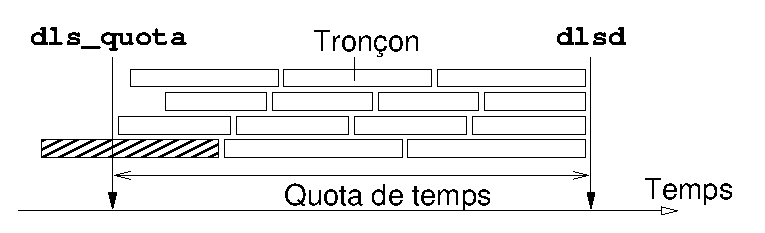
\includegraphics[width=250pt]{bilder/quota_fr}
 \end{center}
 \caption{Conformit\'e avec les quotas de temps}
 \label{fig:quota}
\end{figure}

Puisque le daemon DLS quota ne peut supprimer que des tron\c cons\index{chunk} entiers,
une suppression successive serait impossible, si les donn\'ees acquises
pour un canal consistaient seulement en un tron\c con unique.
C'est pourquoi, il faut garantir qu'il existe toujours plusieurs petits tron\c cons,
m\^eme si le processus d'acquisition dlsd n'a pas \'et\'e interrompu.

Par cons\'equent, le processus d'acquisition dls surveille les
crit\`eres de quota pour lui-m\^eme.  Lorsque les quotas sont
activ\'es, il s'assure que suffisament de tron\c cons individuels sont
produits au sein de la zone critique (\autoref{fig:quota}), Dans ce
but, il d\'ecoupe chaque ensemble de quota en portions \'egales et
commence ind\'ependament un nouveau tron\c con d\`es qu'un de ces
crit\`eres plus fins est d\'epass\'e.

Comme l'ach\`evement d'un tron\c con\index{chunk} peut \^etre tr\`es
co\^uteux en temps, ce qui est incompatible avec les contraintes
temps-r\'eel du processus d'acquisition dlsd, un processus d\'edi\'e
est g\'en\'er\'e pour enregistrer les donn\'ees acquises restantes. Ce
``processus de nettoyage''\index{clean-up process} va enregistrer
maintenant toutes les donn\'ees du tron\c con courant, tandis que le
processus d'acquisition s'en d\'ebarasse et s'occupe de l'acquisition
des donn\'ees du nouveau tron\c con qui commence.  Apr\`es
l'ach\`evement du ``vieux'' tron\c con, le processus de nettoyage
s'arr\^ete automatiquement.


%------------------------------------------------------------------------------

\subsection{Messages depuis la source de donn\'ees}
\label{sec:dlsd_logger_msg}

La source de donn\'ee peut -- en plus des donn\'ees mesur\'ees --
envoyer des messages\index{messages} \`a n'importe quel moment.  Ces
messages contiennent des notes de l'utilisateur qui doivent \^etre
incorpor\'ees dans le flux de donn\'ees, des avertissements ou des
conditions d'erreurs.  Les messages sont parmi les types suivants:

\begin{description}

\item[info] - Information qui concerne seulement le processus d'acquisition courant.

\item[warn] - Un avertissement (warning) en provenance de la source de donn\'ees.

\item[error] - Une erreur s'est produite dans la source de donn\'ees.

\item[crit\_error] - Une erreur rendant difficile ou impossible la suite des op\'erations
  s'est produite dans la source des donn\'ees.

\item[broadcast] - Un message pour tous les processus qui sont actuellement
  connect\'es \`a la source de donn\'ees.

\end{description}

Un message est toujours envoy\'e par la source de donn\'ees sous la
forme d'une balise XML unique, dont le titre inclu le type de message.
En outre, le titre contient un attribut \textit{time} qui indique
l'horodatage du message en secondes et - en fonction du message - un
attribut \textit{text}, qui ne sera pas \'evalu\'e par dlsd.

Une balise typique de message ressemblera \`a ceci:

\begin{lstlisting}
<broadcast time="1093072549.866241" text="test message"/>
\end{lstlisting}

Le processus d'acquisition dlsd enregistre les messages dans le
sous-r\'epertoire \textit{messages} du r\'epertoire de la t\^ache
(voir \autoref{sec:data_msg}).  De la m\^eme mani\`ere que les
donn\'ees mesur\'ees, les messages sont organis\'ees en tron\c
cons. Cependant, le concept de tron\c con est l\'eg\`erement
diff\'erent ici: les tron\c cons contiennent des messages discontinus
dans le temps et sont cr\'e\'es uniquement pour faciliter
ult\'erieurement la suppression d'intervalle de temps dans les messages.

%------------------------------------------------------------------------------

\subsection{Traitement des signaux UNIX}
\label{sec:dlsd_logger_signals}

Les signaux UNIX\index{signal processing} suivants sont trait\'es par
le processus d'acquisition dlsd:

\begin{description}

\item[SIGINT/SIGTERM]
  Le processus d'acquisition doit se terminer. Aussit\^ot, il met fin
  \`a la connection vers la source de donn\'ees et sauvegarde les
  donn\'ees encore en m\'emoire sur le disque dur. Ceci peut prendre
  quelques secondes, car beaucoup de fichiers ont potentiellement
  besoin d'\^etre \'ecrits.  Si aucune erreur ne se produit pendant
  l'op\'eration, le processus se terminera avec la valeur de retour 0.

\item[SIGHUP]
  Quand le processus d'acquisition re\c coit ce signal, il doit relire
  son fichier de sp\'ecifications. Par cons\'equent, il v\'erifiera
  imm\'ediatement, - en fonction des nouvelles sp\'ecifications -, s'il
  doit continuer \`a acqu\'erir des donn\'ees. Sinon, il entamera une
  proc\'edure d'arr\^et comme dans le cas de \textit{SIGINT} ou
  \textit{SIGTERM}.  Autrement, il enverra potentiellement les
  sp\'ecifications modifi\'ees \`a la source de donn\'ees et
  continuera \`a acqu\'erir des donn\'ees apr\`es confirmation (voir
  \autoref{sec:dlsd_logger_comm}) des nouvelles conditions.

\item[SIGCHLD]
  Un ``processus de nettoyage''\index{clean-up process} (voir
  \autoref{sec:dlsd_logger_quota}) s'est achev\'e. Il sera seulement
  enregistr\'e via \textit{syslogd}\index{syslogd}.

\item[SIGSEGV et autres]
  Le traitement est similaire \`a celui du processus parent (voir
\autoref{sec:dlsd_mother_signals}).

\end{description}

%------------------------------------------------------------------------------

\chapter{Le r\'epertoire de donn\'ees DLS}
\label{sec:data}

Toutes les donn\'ees persistentes du syst\`eme DLS sont organis\'ees
dans \textit{les r\'epertoires de donn\'ees DLS }\index{DLS data
  directory}. La structure de base est indiqu\'ee dans
\autoref{fig:dls_data}.

\begin{figure}[htb]
  \begin{center}
    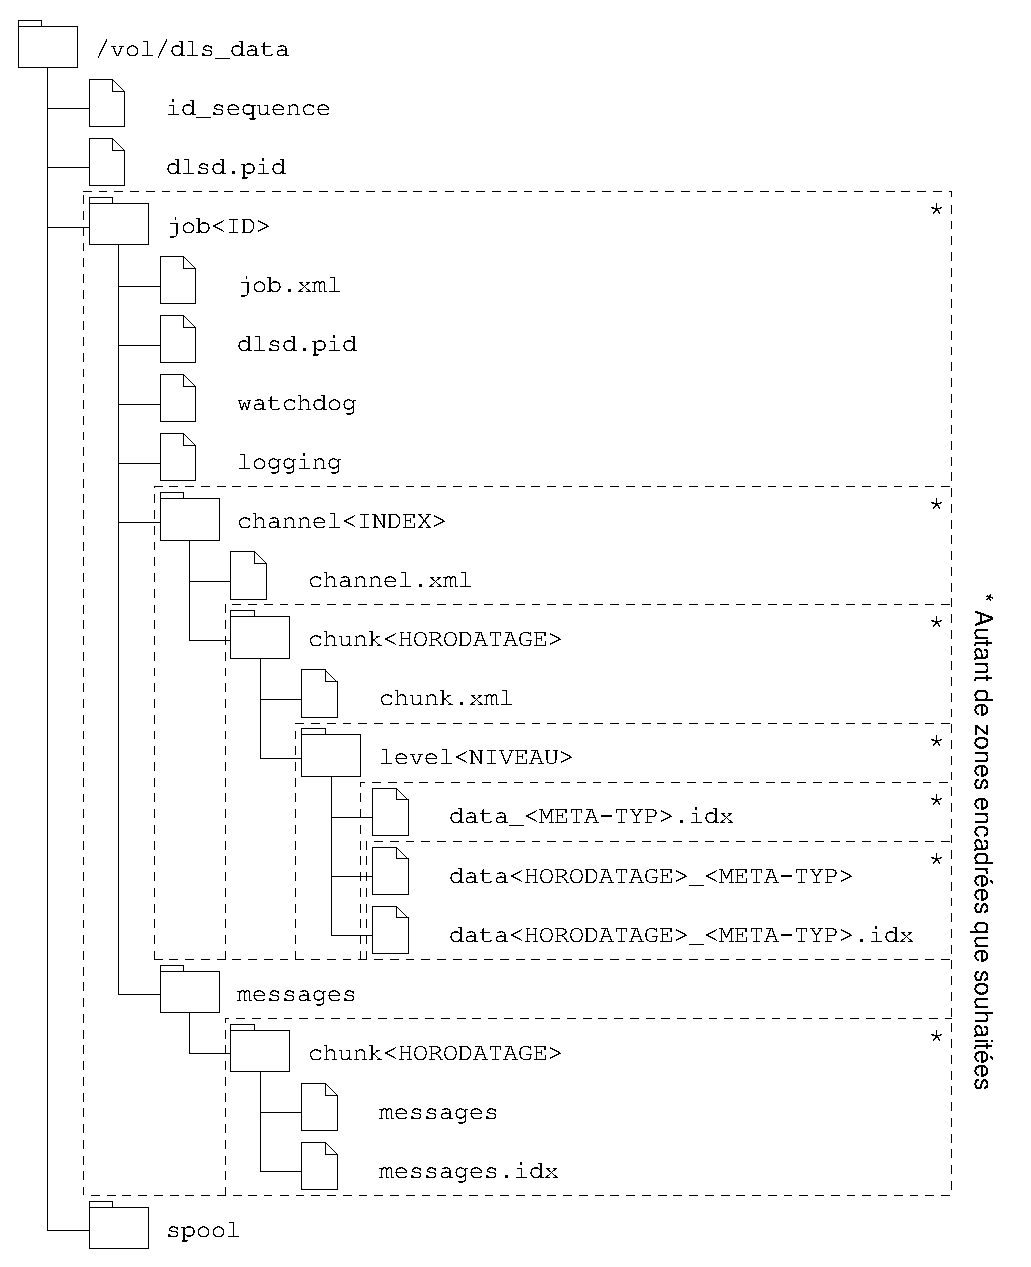
\includegraphics[width=300pt]{bilder/dls_data_fr}
  \end{center}
  \caption{Structure du r\'epertoire de donn\'ees DLS}
  \label{fig:dls_data}
\end{figure}

%------------------------------------------------------------------------------

\section{R\'epertoire racine}
\label{sec:data_root}

Le r\'epertoire racine est le r\'epertoire de niveau le plus \'elev\'e
au sein de l'arborescence de donn\'ees DLS.  La plupart des fichiers
qui s'y trouvent, appartiennent au processus parent dlsd. De plus, le
r\'epertoire racine comprend tous les r\'epertoires des t\^aches
(voir \autoref{sec:data_jobs}).

Fichiers et sous-r\'epertoires dans le r\'epertoire racine:

\begin{description}

\item[id\_sequence] Ce fichier contient le prochain identifiant (ID)
  disponible pour une t\^ache, sous la forme d'un nombre en ASCII. Il
  est n\'ecessaire \`a DLS Manager lors de la cr\'eation d'une
  nouvelle t\^ache. DLS Manager lit l'identifiant, l'utilise pour la
  nouvelle t\^ache, puis l'incr\'emente, avant d'\'ecrire le nouveau
  identifiant dans le fichier.

\item[dlsd.pid] C'est le fichier \textit{PID}\index{PID files} du
  processus parent dlsd (voir \autoref{sec:apx_pid}). Il est automatiquement
  cr\'e\'e \`a l'ex\'ecution et indique qu'un processus parent dlsd est en cours
  d'ex\'ecution.

\item[jobXXX] Chaque r\'epertoire de t\^ache est pr\'esent dans le
  r\'epertoire racine DLS.  Le nom est toujours \textit{job}, suivit
  par l'identifiant de t\^ache. Voir \autoref{sec:data_jobs}.

\item[spool]
  C'est le r\'epertoire de file d'attente du processus parent dlsd.
  Une description est donn\'ee dans \autoref{sec:dlsd_mother_spooling}.

\end{description}


%------------------------------------------------------------------------------

\section{R\'epertoires de t\^aches}
\label{sec:data_jobs}

Pendant le fonctionnement en cours, chaque r\'epertoire de t\^ache
(\textit{job\textless ID\textgreater}) est trait\'e par un processus
d\'edi\'e d'acquisition dlsd.. Ce dernier lit ses sp\'ecifications et
\`a partir de l\`a, y \'ecrit \'egalement les donn\'ees acquises.

Fichiers et r\'epertoires dans le r\'epertoire de t\^ache:

\begin{description}

\item[job.xml]
  Le fichier central des sp\'ecifications de la t\^ache.  Il contient
  les sp\'ecifications de la t\^ache et celles des canaux.  S'il est
  \'edit\'e alors que le processus d'acquisition correspondant est en
  cours d'ex\'ecution, une commande de mise en file d'attente (voir
  \autoref{sec:dlsd_mother_spooling}) doit \^etre g\'en\'er\'ee pour
  que le processus adopte les nouvelles sp\'ecifications. DLS Manager
  le fait automatiquement.

  Les sp\'ecifications sont dans le format XML et contiennent les informations suivantes
  (dont l'ordre est obligatoire~!):

\begin{lstlisting}
<dlsjob>
 <description text="`\textit{description}`"/>
 <state name="`\textit{(}`running`\textit{|}`paused`\textit{)}`"/>
 <source address="`\textit{IP address or host name}`"/>
 <quota size="`\textit{data quota}`" time="`\textit{time quota}`"/>
 <trigger parameter="`\textit{trigger parameter}`"/>

 <channels>
  <channel name="`\textit{channel name}`"
   frequency="`\textit{sampling frequency}`"
   block_size="`\textit{block size}`"
   meta_mask="`\textit{meta mask}`"
   meta_reduction="`\textit{meta reduction ratio}`"
   format="`\textit{compression format}`"
   mdct_block_size="`\textit{MDCT block size}`"
   mdct_accuracy="`\textit{MDCT accuracy}`"
   type="`\textit{data type}`"/>
 </channels>
</dlsjob>
\end{lstlisting}

Les attributs \textit{mdct\_block\_size} et \textit{mdct\_accuracy} sont
n\'ecessaires uniquement si le format de compression choisi est
MDCT (voir \autoref{sec:comp_mdct}).

Les sp\'ecifications peut \^etre \'edit\'ees avec DLS Manager. Les param\`etres
individuels sont d\'ecrits dans \autoref{sec:manager_job_create} et
\autoref{sec:manager_channels_edit}.

\item[Chien de garde et journalisation]
  Deux fichiers vides sont utilis\'es pour la surveillance des
  processus d'acquisitions dls par DLS Manager. Si un processus
  d'acquisition est en cours d'ex\'ecution pour un r\'epertoire de
  t\^ache, il modifiera chaque seconde l'horodatage du fichier
  \textit{watchdog}.  Si le processus est aussi en train d'acqu\'erir
  des donn\'ees, il proc\`edera de la m\^eme mani\`ere avec le fichier
  \textit{logging}.  DLS Manager v\'erifie r\'eguli\`erement
  l'horodatage de ces fichiers et peut ainsi conna\^itre l'\'etat du
  processus d'acquisition et en informer l'utilisateur.


\item[dlsd.pid]
  C'est le fichier \textit{PID}\index{PID files} du processus d'acquisition
  (voir \autoref{sec:apx_pid}). Il est automatiquement cr\'e\'e
  au moment de l'ex\'ecution et indique que le processus d'acquisition
  dlsd est en cours de fonctionnement.

\item[channelXXX]
  Les donn\'ees acquises continuent d'\^etre organis\'ees en canaux
  qui ont chacun leur propre r\'epertoire (voir \autoref{sec:data_channels}).
  L'index dans le nom du r\'epertoire de canal correspond \`a l'index de canal
  que la commande \textit{\textless rk\textgreater} a renvoy\'ee
  lors de l'\'enum\'eration des canaux de la source de donn\'ees
  pendant la s\'equence de d\'emarrage du processus parent dlsd
  (voir \autoref{sec:dlsd_logger_comm}).

\item[messages]
  Chaque processus d'acquisition stocke dans ce r\'epertoire, les
  messages qu'il a re\c cu de la source pendant l'acquisition des
  donn\'ees.  Si le r\'epertoire est manquant, le processus le
  cr\'eera au moment requis.  De mani\`ere similaire aux donn\'ees
  mesur\'ees, les messages sont organis\'es en canaux. Voir
  \autoref{sec:data_msg}.

\end{description}


%------------------------------------------------------------------------------

\section{R\'epertoire de canal}
\label{sec:data_channels}

L'ensemble des donn\'ees acquises pour un canal donn\'e sont rang\'ees
dans le r\'epertoire de canal (\textit{channel\textless INDEX\textgreater}).
Un r\'epertoire de canal est assign\'e en permanence \`a un canal sp\'ecifique de la source.
Les propri\'et\'es du canal sont d\'ecrites dans le fichier \textit{channels.xml}
qui contient:

\begin{lstlisting}
<dlschannel>
 <channel name="`\textit{channel name}`" index="`\textit{Index}`"
  unit="`\textit{unit}`" type="`\textit{Data type}`"/>
</dlschannel>
\end{lstlisting}

Le fichier sert non seulement \`a d\'ecrire les donn\'ees dans les r\'epertoires de
tron\c cons mais aussi par le processus d'acquisition dlsd
\`a chaque fois qu'une nouvelle acquisition de donn\'ees
doit \^etre faite dans un r\'epertoire de canal.
Ceci ne doit avoir lieu que si les caract\'eristiques du canal
(name, index, unit and type) n'ont pas chang\'e.

%------------------------------------------------------------------------------

\section{R\'epertoire de tron\c cons}
\label{sec:data_chunks}

Les donn\'ees acquises pour un canal sont organis\'ees en
\textit{tron\c cons} (en anglais \textit{chunks})
(\textit{chunk\textless TIME\textgreater}). Un tron\c con\index{chunk}
est une s\'erie de donn\'ees dont l'acquisition est termin\'ee
et qui a \'et\'e obtenue avec les m\^emes sp\'ecifications de canal
depuis une origine de temps donn\'ee.
L'horodatage du r\'epertoire est le m\^eme que celui de la premi\`ere donn\'ee
du tron\c con.
Les propri\'et\'es du tron\c con sont d\'ecrites dans le fichier
\textit{chunk.xml} qui contient:

\begin{lstlisting}
<dlschunk>
 <chunk sample_frequency="`\textit{Fr\'equence d'\'echantillonnage}`"
  block_size="`\textit{Taille de bloc pour les donn\'ees}`"
  meta_mask="`\textit{M\'eta-Masque}`"
  meta_reduction="`\textit{M\'eta-r\'eduction}`"
  format="`\textit{Format de compression}`"
  mdct_block_size="`\textit{Taille de block MDCT}`"
  mdct_accuracy="`\textit{Pr\'ecision MDCT}`"
  architecture="`\textit{Architecture (Endianess)}`"/>
</dlschunk>
\end{lstlisting}

Les attributs \textit{mdct\_*} existent si et seulement si
le format de compression selectionn\'e est MDCT (voir \autoref{sec:comp_mdct}).

Dans chaque r\'epertoire de tron\c con, les donn\'ees sont rang\'ees
dans les r\'epertoires correspondant \`a leur m\'eta-niveau
(les donn\'ees g\'en\'eriques sont dans le r\'epertoire \textit{level0},
les donn\'ees du premier m\'eta-niveau sont dans le r\'epertoire \textit{level1}
et ainsi de suite).

%------------------------------------------------------------------------------

\section{R\'epertoire de donn\'ees}
\label{sec:data_data}

Les r\'epertoires de donn\'ees (\textit{level\textless meta
  level\textgreater}), qui repr\'esent le tri des donn\'ees en
fonction de leur m\'eta-niveau, sont arrang\'e en bas de la hierarchie
des r\'epertoires.  Les fichiers de donn\'ees et les fichiers d'index
associ\'es sont d\'etaill\'e ci-dessous:

\paragraph{Fichier de donn\'ees}
Les fichiers de donn\'ees contiennent les donn\'ees mesur\'ees acquises. Ils
sont cr\'e\'es s\'epar\'ement pour chaque m\'eta-type. C'est pourquoi,
le fichier suit la convention de nommage suivante:

\begin{quote}
  \textit{data\textless HORODATAGE\textgreater\_\textless METATYPE\textgreater}
\end{quote}

L'horodatage dans le nom de fichier est l'horodatage de la premi\`ere
valeur dans le premier bloc du fichier.

Dans le r\'epertoire \textit{level0}, le m\'eta-type est toujours
\textit{gen} (``generic'').

Les fichiers de donn\'ees ont une structure XML simple.  Chaque bloc
de donn\'ee appara\^it dans une balise \textit{\textless
  d\textgreater}.  Celle-ci contient l'horodatage de la premi\`ere
valeur du bloc dans l'attribut \textit{t} (``time''), le nombre de
valeurs compress\'ees dans l'attribut \textit{s} (``size'') et les
donn\'ees cod\'ees dans l'attribut \textit{d}(``data'').

Les fichiers de donn\'ees ont une taille maximale d\'efinie.  Lorsque
le processus d'acquisition dlsd est sur le point de d\'epasser cette
taille en ajoutant un bloc, il d\'ebutera \`a la place un nouveau
fichier de donn\'ee.

Les param\`etres qui ont \'et\'e finalement utilis\'es pour
l'acquisition de donn\'ees et le type de compression employ\'e ne
peuvent \^etre d\'etermin\'es qu'en consultant les fichiers de
description de haut-niveaux \textit{chunk.xml} et
\textit{channel.xml}.

\paragraph{Fichiers d'index}
Les fichiers d'index sont des fichiers binaires avec une longueur d'enregistrement fixe, qui sont assign\'es \`a un fichier de donn\'ees.
Ils fournissent des informations qui peuvent \^etre lues tr\`es rapidement,
\`a propos des blocs dans les fichiers correspondants.
La convention de nommage est similaire \`a celle des fichiers de donn\'ees, mais
avec un suffixe suppl\'ementaire.

\begin{quote}
  \textit{data\textless HORODATAGE\textgreater\_\textless METATYPE\textgreater.idx}
\end{quote}

Les enregistrements du fichier d'index correspondent toujours \`a
un bloc dans le fichier de donn\'ees. La structure d'un enregistrement
est expliqu\'ee dans \autoref{fig:dls_data_index}.

\begin{figure}[htb]
  \begin{center}
    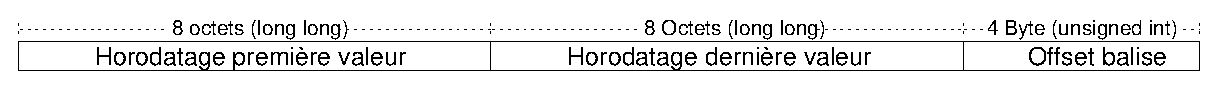
\includegraphics[height=15pt]{bilder/dls_data_index_fr}
  \end{center}
  \caption{Enregistrement du fichier d'index}
  \label{fig:dls_data_index}
\end{figure}

Chaque enregistrement contient 20 octets. Les 8 premiers octets
contiennent l'horodatage en microsecondes (type \textit{long long}) de
la premi\`ere valeur du bloc.  Les 8 octets suivants correspondent de
mani\`ere similaire \`a l'horodatage de la derni\`ere valeur dans le
bloc. Enfin, Les 4 derniers octets sont le d\'ecalage (type
\textit{unsigned int}) de la balise du bloc dans le fichier de
donn\'ee, c'est \`a dire la position du caract\`ere initial
``\textit{\textless}''.

\paragraph{Fichier d'index globaux}
Les fichiers d'index globaux permettent de d\'eterminer plus
facilement les intervalles de temps des fichiers individuels de
donn\'ees pour un m\'eta-type particulier. Leur convention de nommage
est:

\begin{quote}
  \textit{data\_\textless METATYPE\textgreater.idx}
\end{quote}

Un enregistrement dans un fichier d'index global correspond toujours
\`a un fichier de donn\'ee du m\^eme m\'eta-type.  La structure d'un
enregistrement est expliqu\'ee dans \autoref{fig:dls_data_index_glob}.

\begin{figure}[htb]
  \begin{center}
    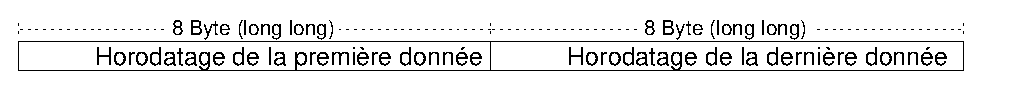
\includegraphics[height=15pt]{bilder/dls_data_index_glob_fr}
  \end{center}
  \caption{Enregistrement d'un fichier d'index global}
  \label{fig:dls_data_index_glob}
\end{figure}

Un enregistrement dans un fichier d'index global fait toujours 16
octets de long. Les 8 premiers octets correspondent \`a l'horodatage
en microsecondes (type \textit{long long}) de la premi\`ere valeur
dans le fichier de donn\'ees, les 8 derniers octets \`a l'horodatage
de la derni\`ere valeur dans le fichier de donn\'ees.

Si une donn\'ee vient juste d'\^etre ajout\'ee dans un fichier de
donn\'ee, l'horodatage de l'enregistrement correspondant (le dernier)
dans le fichier d'index global sera 0.  Dans ce cas l'horodatage
recherch\'e doit \^etre v\'erifi\'e en lisant le dernier
enregistrement dans le fichier d'index des donn\'ees.  D\`es que
l'acquisition des donn\'ees est termin\'e dans le fichier de donn\'ee,
le second horodatage donnera la valeur ``correcte''.

%------------------------------------------------------------------------------

\section{R\'epertoire de messages}
\label{sec:data_msg}

Les messages en provenance de la source de donn\'ees sont stock\'es
dans le r\'epertoire de messages (\textit{messages}) dans des tron\c
cons s\'epar\'es. Tous les r\'epertoires de tron\c cons sont
d\'esign\'es par

\begin{quote} \textit{chunk\textless HORODATAGE\textgreater} \end{quote}

o\`u l'horodatage correspond au premier message enregistr\'e dans ce
r\'epertoire. Au sein des r\'epertoires, il y a toujours seulement
deux fichiers: le fichier des messages et le fichier d'index
associ\'e.

\paragraph{Fichiers de messages}
Un fichier avec des messages venant de la source de donn\'ees est
toujours nomm\'e \textit{messages}.  Les messages de la source de
donn\'ees sont enregistr\'es sans transformation dans ce fichier,
aussi il contient de simples balises XML qui correspondent aux
messages respectifs (voir \autoref{sec:dlsd_logger_msg})).

\paragraph{Fichiers d'index de messages}
Le fichier d'index \textit{messages.idx} appartient au fichier des
messages et sert \`a activer le chargement rapide des
messages pour un intevalle de temps donn\'e sans devoir lire
l'int\'egralit\'e des messages.

Un enregistrement dans le fichier d'index correspond \`a un message
dans le fichier de message. La structure d'un enregistrement est
d\'ecrite dans \autoref{fig:dls_data_index_msg}.

\begin{figure}[htb]
  \begin{center}
    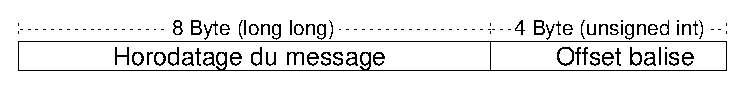
\includegraphics[height=15pt]{bilder/dls_data_index_msg_fr}
  \end{center}
  \caption{Enregistrement d'index de message}
  \label{fig:dls_data_index_msg}
\end{figure}

%------------------------------------------------------------------------------

\chapter{DLS Manager}
\label{sec:manager}

\textit{DLS Manager}\index{DLS Manager} est une interface graphique
utilisateur pour configurer les t\^ache
d'acquisition\index{measurement job} dans un r\'epertoire de donn\'ees
DLS. En outre, il sert au contr\^ole et \`a la surveillance des
processus d'acquisition en cours d'\'ex\'ecution.

DLS Manager est d\'emarr\'e par la commande \texttt{dls\_ctl}.

De la m\^eme mani\`ere que dlsd, le param\`etre \texttt{-d} dans la
ligne de commande permet de sp\'ecifier le r\'epertoire de donn\'ees
DLS dans lequel le programme doit travailler (voir
\autoref{sec:apx_cmd_dlsctl}).

Quand le programme DLS Manager d\'emarre, il effectue automatiquement
des v\'erifications:

\begin{itemize}
\item Si le r\'epertoire de donn\'ee DLS est vide, il demande \`a
  l'utilisateur si une structure valide de r\'epertoires doit \^etre
  cr\'e\'ee \`a l'int\'erieur de celui-ci.
\item S'il n'y a pas d'instance du d\'emon dlsd en cours d'ex\'ecution,
  il demande \`a l'utilisateur s'il veut en d\'emarrer une nouvelle.
  \end{itemize}

%------------------------------------------------------------------------------

\section{Fen\^etre principale}

\autoref{fig:dls_ctl_main} pr\'esente la fen\^etre principale de
DLS Manager, qui s'affiche lorsque le programme est d\'emarr\'e.


\begin{figure}[tbh]
  \begin{center}
    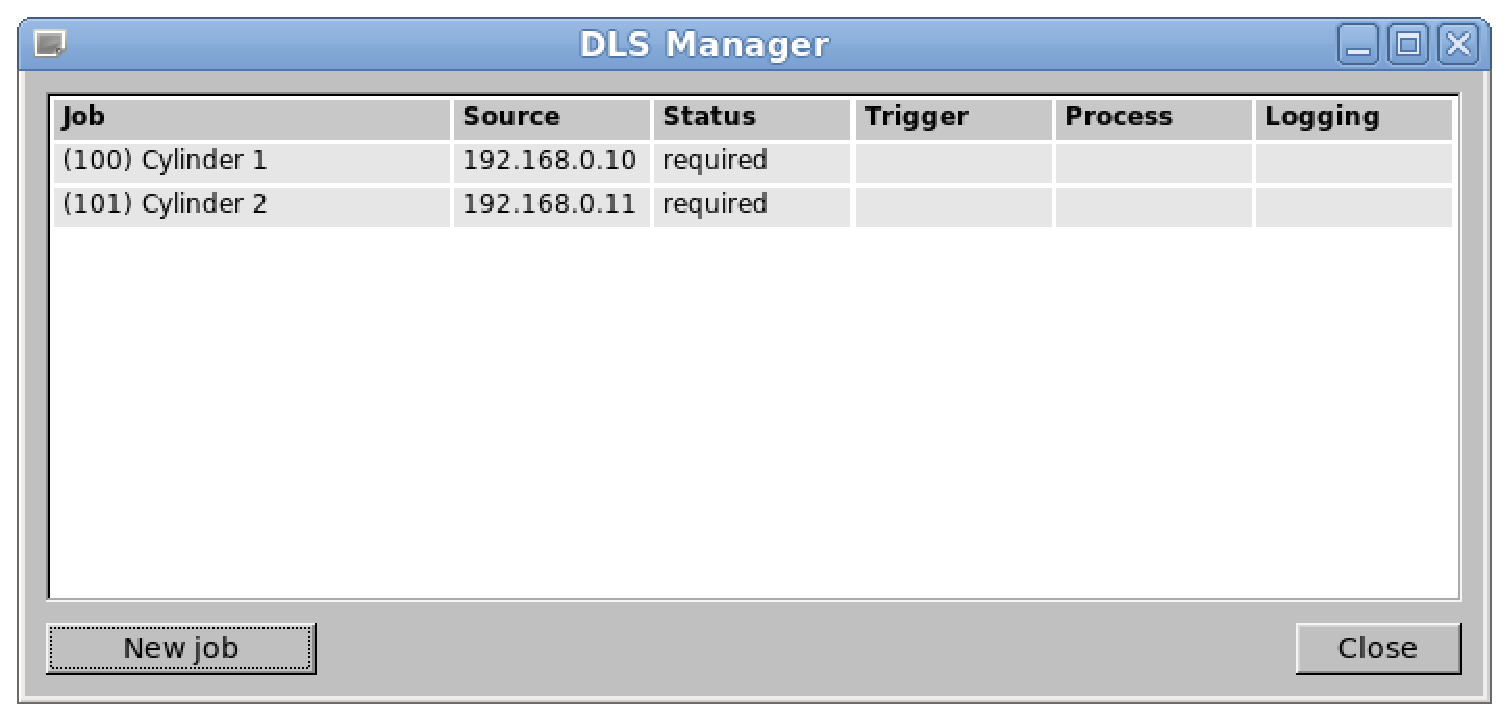
\includegraphics[width=300pt]{bilder/ctl_main_en}
  \end{center}
  \caption{Fen\^etre principale de DLS Manager}
  \label{fig:dls_ctl_main}
\end{figure}

%------------------------------------------------------------------------------

\subsection{Description}

Dans la fen\^etre principale, les t\^aches d'acquisition\index{measurement job}
individuelles sont affich\'ees sous forme de lignes dans un tableau.
Les informations suivantes sont disponibles dans les colonnes:

\begin{description}
\item[Description]
  La description de la t\^ache est arbitraire et peut \^etre modifi\'ee
  \`a tout moment. L'ID est un nombre fixe automatiquement attribu\'e
  au moment de la cr\'eation de la t\^ache. Toutes les donn\'ees de la
  t\^ache sont enregistr\'ees dans le r\'epertoire de donn\'ees DLS
  dans le sous-r\'epertoire \textit{job\textless ID\textgreater}.

\item[Source]
  Le nom d'h\^ote ou l'adresse IP du serveur qui sert de source de
  donn\'ees.  Sur ce dernier un serveur de contr\^ole et commandes
  doit \^etre accessible via le port TCP 2345.  La source doit \^etre
  obligatoirement choisie au moment de la cr\'eation de la t\^ache et
  elle ne peut plus \^etre modifi\'ee par la suite.

\item[Status]
  Le status de la t\^ache selectionn\'ee par l'utilisateur: ``started'',
  quand l'acquisition de donn\'ees est d\'emar\'ee, sinon ``stopped''.

\item[Trigger].
  Le param\`etre de la source de donn\'ee qui servira de g\^achette
  pour le processus d'acquisition de donn\'ees. Lorsque qu'un
  param\`etre de g\^achette est selectionn\'e, les donn\'ees sont
  acquises seulement lorsque la g\^achette vaut 1.

\item[Process]
  Indique si un processus d'acquisition est en cours d'ex\'ecution pour
  cette t\^ache. Rien n'est affich\'e quand la t\^ache est arr\^et\'ee.

\item[Acquisition]
  Si une g\^achette a \'et\'e configur\'ee, vous pouvez voir ici si
  elle est activ\'ee.  Sans g\^achette, l'acquisition de donn\'ees est
  toujours activ\'ee quand le processus d'acquisision est en cours
  d'ex\'ecution.

\end{description}

%------------------------------------------------------------------------------

\subsection{Utilisation}

\begin{itemize}

\item Le lignes contenant les t\^aches individuelles peut \^etre
  selectionn\'ees avec le curseur de la souris.

\item Quand une t\^ache est s\'electionn\'ee, un bouton \textit{start}
  (démarrer) ou \textit{stop} est affich\'e pour contr\^oler
  l'acquisition des donn\'ees.

\item Un double-click sur une t\^ache ouvre un dialogue
  pour \'editer la t\^ache correspondante (voir
  \autoref{sec:manager_job_edit}).

\item Le bouton ``Close'' termine le programme.

\end{itemize}

%------------------------------------------------------------------------------

\section{Les dialogues ``Create job'' et ``Change job''}
\label{sec:manager_job_create}

\autoref{fig:dls_ctl_change} montre le dialogue pour
cr\'eer ou modifier une t\^ache d'acquisition. Elle s'affiche apr\`es
avoir cliqu\'e sur le bouton ``New job'' de la fen\^etre principale ou
le bouton ``Change'' dans le dialogue ``Edit job''.  La
seule diff\'erence entre les deux est que la source de donn\'ees ne
peut \^etre modifi\'ee que lors de la cr\'eation de la t\^ache.

\begin{figure}[tbh]
  \begin{center}
    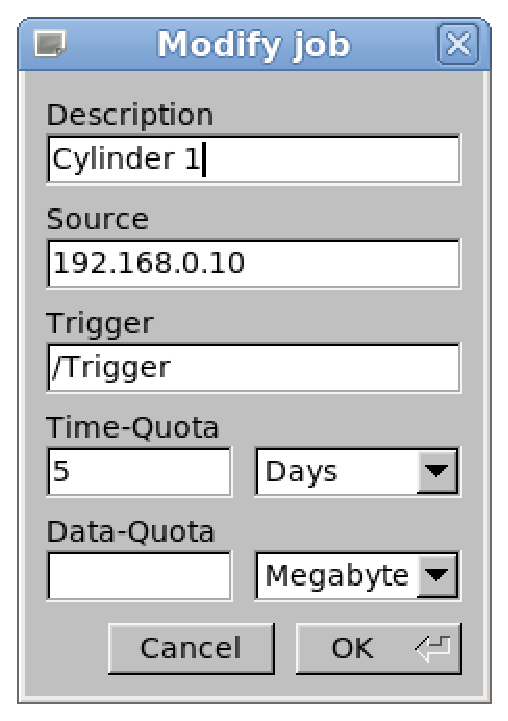
\includegraphics[width=100pt]{bilder/ctl_change_en}
  \end{center}
  \caption{Dialogue pour cr\'eer ou modifier une t\^ache
    d'acquisition}
  \label{fig:dls_ctl_change}
\end{figure}

%------------------------------------------------------------------------------

\subsection{Description}

Les diff\'erents champs du dialogue permettent \`a l'utilisateur
d'indiquer les particularit\'es de la t\^ache d'acquisition:

\begin{description}

\item[Description]
  C'est un nom arbitraire pour la t\^ache d'aquisition qui sert seulement
pour simplifier l'identification.

\item[Source]
  L'adresse de la source de donn\'ees. \c Ca peut \^etre un nom
  d'h\^ote ou une adresse IP. Si un nom d'h\^ote est utilis\'e, il
  faut qu'il puisse \^etre r\'esolu par dlsd au moment de
  l'ex\'ecution.  L'h\^ote sp\'ecifi\'e doit fournir une source de
  donn\'ee pour l'acquisition et pour les canaux additionnels via le
  protocole correspondant (see \autoref{sec:manager_channels_add}).

\item[Trigger]
  Le nom du param\`etre qui servira de g\^achette.
  Si un param\`etre de g\^achette a \'et\'e s\'electionn\'e ici,
  les donn\'ees ne seront acquises que si ce param\`etre a la valeur 1.
  Si le champ d'entr\'ee est vide, aucune g\^achette n'est utilis\'ee.

\item[Time quota]
  Le quota de temps (la dur\'ee maximale de r\'etention des donn\'ees
  acquises voir \autoref{sec:dlsd_logger_quota}) peut \^etre
  indiqu\'e ici sous la forme d'un entier et d'une unit\'e de temps
  (jours, heures, minutes ou secondes).  Si le champ d'entr\'ee est
  vide, alors aucun quota de temps n'est appliqu\'e.

\item[Data quota]
  Le quota de stockage (le volume maximal de stockage r\'eserv\'e pour
  les donn\'ees acquises) peut \^etre indiqu\'e sous la forme d'un
  entier et d'une unit\'e de taille.  Si le champ d'entr\'ee est
  vide, alors aucun quota de stockage n'est appliqu\'e.

\end{description}

%------------------------------------------------------------------------------

\subsection{Utilisation}

\begin{itemize}

\item Les champs sont v\'erifi\'ees en cliquant sur le bouton ``OK''
  (ou en pressant la touche \textit{Entr\'ee}. S'ils contiennent des
  erreurs, une fen\^etre sera affich\'ee avec les messages exactes des
  erreurs. Autrement, les champs d'entr\'ees sont accept\'es et le
  dialogue est ferm\'e. Si un processus d'acquisition dlsd
  est en cours d'ex\'ecution, il lui sera demand\'e de tenir compte
  des nouvelles sp\'ecifications.

\item Si le bouton ``Cancel'' (Annuler) est cliqu\'e, les champs
  d'entr\'ees sont annul\'es et le dialogue est ferm\'e.

\end{itemize}

%------------------------------------------------------------------------------

\section{Le dialogue ``Edit job''}
\label{sec:manager_job_edit}

\autoref{fig:dls_ctl_edit} montre le dialogue pour \'editer une t\^ache. Elle
s'affiche lors d'un double-clic sur une t\^ache de la fen\^etre principale.

\begin{figure}[tbh]
  \begin{center}
    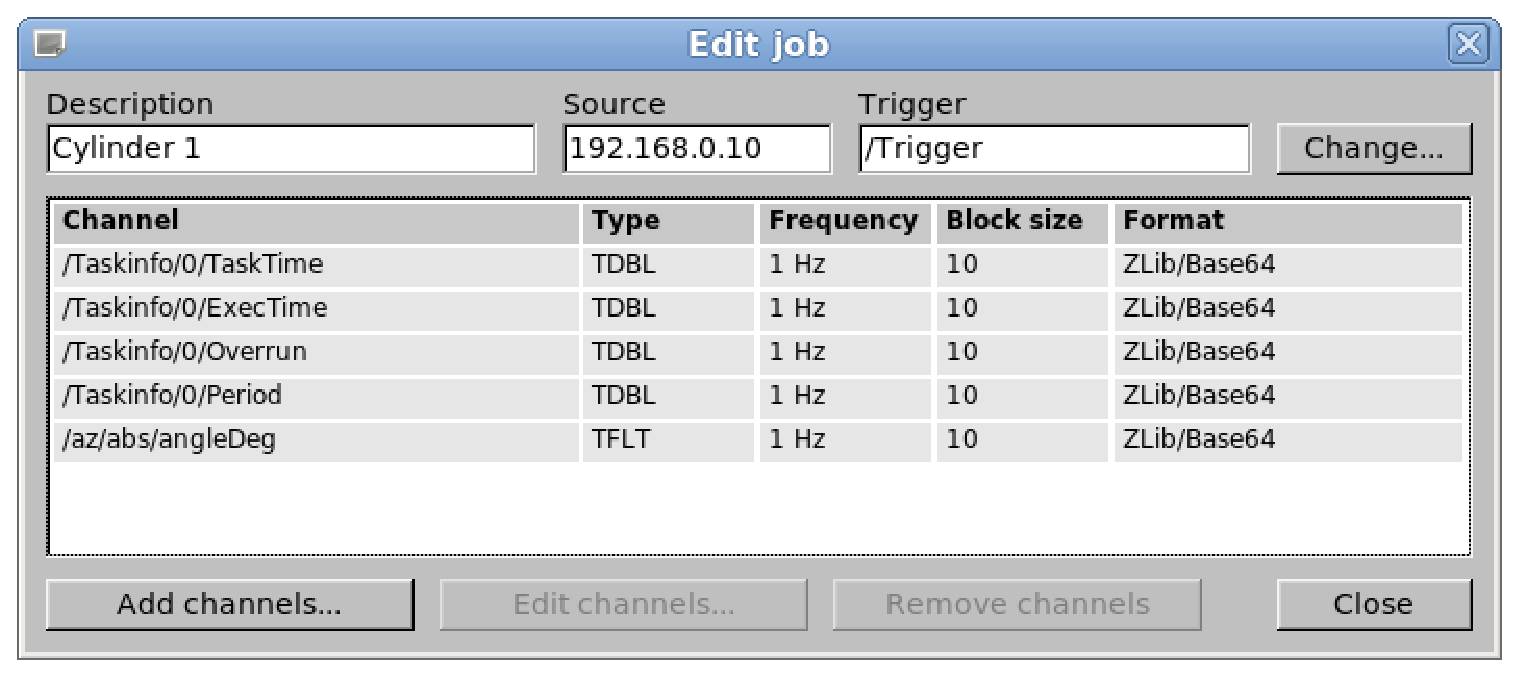
\includegraphics[width=300pt]{bilder/ctl_edit_en}
  \end{center}
  \caption{Dialogue pour \'editer une t\^ache}
  \label{fig:dls_ctl_edit}
\end{figure}

%------------------------------------------------------------------------------

\subsection{Description}

La source des donn\'ees est affich\'ee en haut. En dessous, se trouve la liste des canaux
\`a inclure et leurs param\`etres cl\'es. En particulier:

\begin{description}

\item[Channel]
  Le nom du canal \`a inclure

\item[Type]
  Le type de canal. Un canal peut \^etre de type entier ou virgule
  flottante (voir \autoref{sec:apx_types}).

\item[Scanning frequency]
  La fr\'equence d'\'echantillonnage, c'est-\`a-dire, la fr\'equence
  \`a laquelle les donn\'ees sont enregistr\'ees.

\item[Block size]
  Le nombre de donn\'ees acquises qui doivent \^etre compress\'ees et sauvegard\'es
  ensemble pour former une unit\'e.

\item[Format]
  La m\'ethode de compression (voir \autoref{sec:comp}).

\end{description}

%------------------------------------------------------------------------------

\subsection{Utilisation}

\begin{itemize}

\item le dialogue pour \'editer les caract\'eristiques principales d'une t\^ache
  peut \^etre affich\'e en cliquant sur le bouton ``Change''.

\item Les lignes du tableau des canaux peut \^etre s\'electionn\'ees
  avec le curseur de la souris. Il est alors possible d'utiliser les boutons
  ``Edit channels'' et ``Delete channels''.

\item En pressant les touches \textit{Shift} ou \textit{Ctrl}, vous
  pouvez s\'electionner plusieurs canaux \`a la fois, qui peuvent
  alors \^etre \'edit\'es ou supprim\'es simultan\'ement.

\item Les sp\'ecifications pour un ou plusieurs canaux
  s\'electionn\'es peuvent \^etre \'edit\'ees en cliquant sur les
  boutons ``Edit channels.''  du dialogue suivant.
  Cependant, des conditions sp\'eciales s'appliquent pour \'editer
  plusieurs canaux en parall\`ele (voir
  \autoref{sec:manager_channels_edit_parallel}).

\item Un double clic sur une ligne d'un canal ouvre aussi le
  dialogue pour \'editer les sp\'ecifications du canal
  correspondant.

\item Si le bouton ``Delete channels'' est cliqu\'e, tous les canaux
  s\'electionn\'es sont retir\'es des sp\'ecifications. Cependant les
  donn\'ees acquises restent disponibles.

\item Lorsque le bouton ``Add channels'' est cliqu\'e, le dialogue
  pour ajouter des canaux aux sp\'ecifications s'ouvre
 (see \autoref{sec:manager_channels_add}).

\item Le bouton ``Close'' ferme le dialogue et retourne
  \`a la fen\^etre principale.

\end{itemize}

%------------------------------------------------------------------------------

\section{Le dialogue ``Add channels''}
\label{sec:manager_channels_add}

En cliquant le bouton ``Add channels'' dans le dialogue pour \'editer
une t\^ache, une fen\^etre s'ouvre comme montr\'e dans
\autoref{fig:dls_ctl_add}.  Au m\^eme instant, le programme essaye
d'\'etablir une connexion TCP vers la source de donn\'ees pour
r\'ecup\'erer la liste des canaux.

\begin{figure}[tbh]
  \begin{center}
    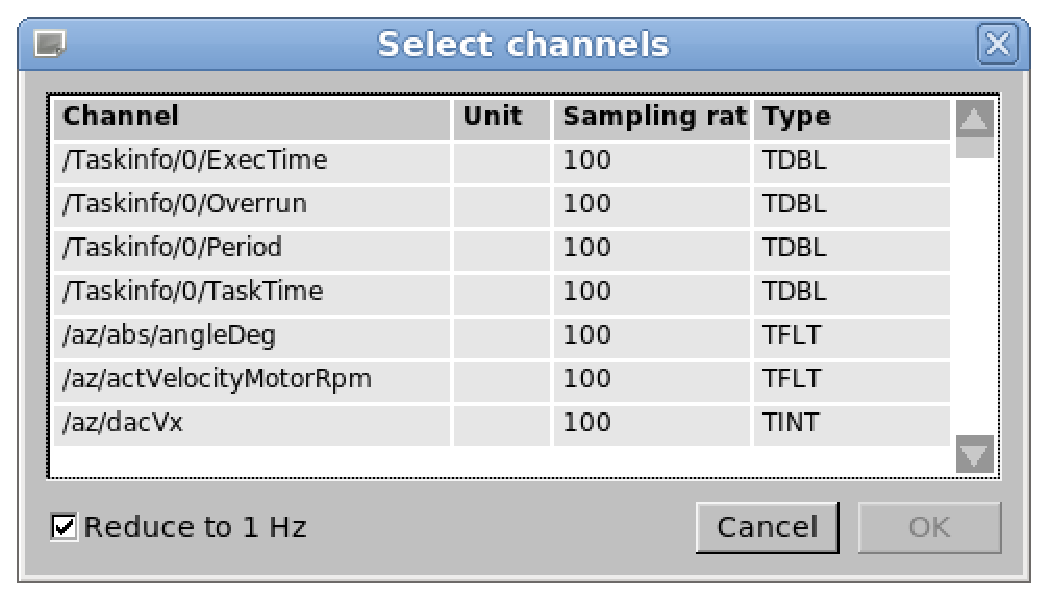
\includegraphics[width=300pt]{bilder/ctl_add_en}
  \end{center}
  \caption{Dialogue pour ajouter des sp\'ecifications de canaux}
  \label{fig:dls_ctl_add}
\end{figure}

%------------------------------------------------------------------------------

\subsection{Description de l'affichage}

\begin{itemize}
\item Tandis qu'il essaye d'\'etablir la connexion avec la source de
  donn\'ee, le message ``Receiving channels\ldots'' s'affiche.  Si
  apr\`es un temps d'attente pr\'e-d\'efini la connexion ne parvient
  toujours pas \`a \^etre \'etablie, une fen\^etre avec le message
  d'erreur correspondant appara\^it et le dialogue se
  ferme.
\item Si la liste des canaux a \'et\'e r\'ecup\'er\'ee avec succ\`es,
  les canaux individuels sont affich\'es dans un tableau.  Le nom du
  canal, l'unit\'e, la fr\'equence maximale d'\'echantillonnage et le
  type de donn\'ee sont affich\'es.
\end{itemize}

%------------------------------------------------------------------------------

\subsection{Utilisation}

\begin{itemize}

\item L'utilisateur peut utiliser le curseur de la souris pour
  s\'electionner les canaux individuels.  En pressant les touches
  \textit{Ctrl} ou \textit{Shift}, il est possible de s\'electionner
  plusieurs canaux \`a la fois.

\item Lorsque le bouton ``OK'' est cliqu\'e, tous les canaux
  s\'electionn\'es sont ajout\'es \`a la liste des sp\'ecifications
  de canaux de la t\^ache.  Si un canal particulier est d\'ej\`a
  disponible, il sera affich\'e dans une fen\^etre avec le message
  d'avertissement correspondant. Les autres canaux seront n\'eanmoins
  ajout\'es. Si des modifications ont \'et\'e faites, le processus
  d'acquisition dlsd en cours d'ex\'ecution adoptera les nouvelles
  sp\'ecifications des canaux.

\item Un clic sur le bouton ``Cancel'' ferme le dialogue
  sans ajouter de nouvelles sp\'ecifications de canaux au t\^ache.

\end{itemize}

%------------------------------------------------------------------------------

\section{Le dialogue ``Edit channels''}
\label{sec:manager_channels_edit}

Le dialogue pour \'editer les sp\'ecifications d'un canal,
tel que montr\'e dans \autoref{fig:dls_ctl_channel} appara\^it lors
d'un double-clic sur la sp\'ecification d'un canal dans le
dialogue pour \'editer une t\^ache, ou bien apr\`es un clic sur le
bouton ``Edit channels'' apr\`es avoir s\'electionn\'e un ou plusieurs
canaux.

\begin{figure}[tbh]
  \begin{center}
    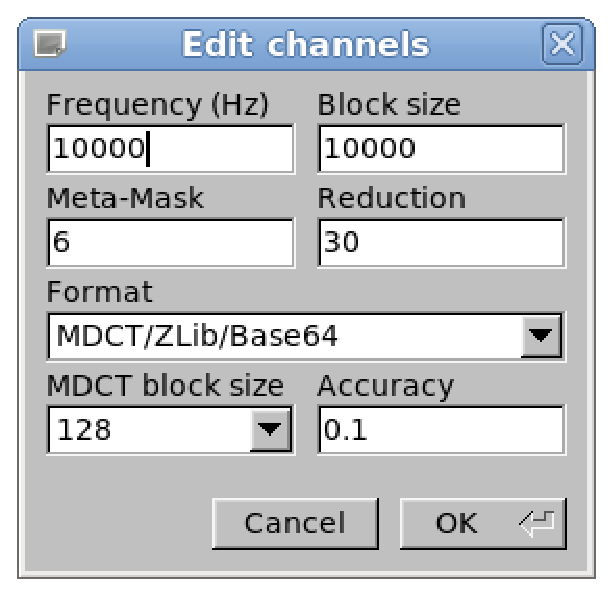
\includegraphics[width=100pt]{bilder/ctl_channel_en}
  \end{center}
  \caption{Dialogue pour \'editer les sp\'ecifications d'un canal}
  \label{fig:dls_ctl_channel}
\end{figure}

%------------------------------------------------------------------------------

\subsection{Description de l'affichage}

Les champs d'entr\'ee suivants sont disponibles pour l'utilisateur
pour param\'etrer les sp\'ecifications d'un canal.

\begin{description}

\item[Sample Rate] Fr\'equence d'\'echantillonnage, c'est-\`a-dire le
  nombre de valeur stock\'ees par seconde. Cette fr\'equence doit
  \^etre un diviseur entier de la fr\'equence maximale
  d'\'echantillonnage du canal concern\'e.

\item[Block Size] Le nombre de valeurs compress\'ees et stock\'ees
  dans un bloc. Plus le bloc est grand, meilleurs sont les
  r\'esultats de la compression, mais plus celle-ci dure longtemps.
  Pour une compression MDCT, la taille de bloc doit \^etre un multiple
  entier de la taille du bloc MDCT.

\item[Meta mask] \textit{Cette valeur n'est actuellement pas
  \'editable}\\ Le m\'eta-masque est un masque binaire qui indique les
  m\'eta-donn\'ees qui sont enregistr\'ees. Voir
  \autoref{sec:dlsd_data_meta}.

\item[Reduction ratio] Le raport de m\'eta-r\'eduction est le nombre
  de valeurs d'un m\'eta-niveau. Voir aussi
  \autoref{sec:dlsd_data_meta}.  Cette valeur ne requi\`ere
  habituellement aucun ajustement.

\item[Format] Le format de compression dans lequel les donn\'ees
  acquises sont compress\'ees avant l'enregistrement.  En fonction de
  la m\'ethode de compression, des param\`etres additionnels ont
  besoin d'\^etre sp\'ecifi\'es.

\item[MDCT block size] Ce param\`etre doit \^etre sp\'ecifi\'e pour
  les m\'ethodes de compression MDCT et se comporte de mani\`ere
  similaire \`a la taille de bloc. Voir \autoref{sec:comp_mdct}.

\item[Accuracy] Certaines m\'ethodes de compression avec pertes
  autorisent la sp\'ecification d'une erreur absolue
  maximale. L'erreur doit toujours \^etre indiqu\'ee dans l'unit\'e du
  canal correspondant.

\end{description}

%------------------------------------------------------------------------------

\subsection{Utilisation}

\begin{itemize}

\item Lorsque le bouton ``OK'' est cliqu\'e, le programme v\'erifie
  tout d'abord la plausibilit\'e des param\`etres.  Si cette
  v\'erification \'echoue, une fen\^etre s'affiche avec le message
  d'erreur ad\'equat.  Autremenent, tous les param\`etres
  sp\'ecifi\'es sont appliqu\'es aux canaux pr\'ealablement
  s\'electionn\'es, et le processus d'acquisision dlsd en cours
  d'ex\'ecution adopte les nouvelles sp\'ecifications des canaux,
  puis le dialogue se ferme.

\item Si le bouton ``Cancel'' est cliqu\'e, les param\`etres sont
  ignor\'es et le dialogue se ferme.

\end{itemize}

%------------------------------------------------------------------------------

\subsection{\'Edition simultan\'ee de plusieurs sp\'ecifications de canaux}

\label{sec:manager_channels_edit_parallel}

Le dialogue pour \'editer les sp\'ecifications des canaux
(\autoref{fig:dls_ctl_channel}) peut aussi \^etre utilis\'e pour
\'editer simultan\'ement plusieurs canaux. Dans ce cas, les
conditions suivantes s'appliquent:

\begin{itemize}
\item Lors de l'ouverture du dialogue, tous les param\`etres
  qui sont identiques pour tous les canaux \`a \'editer seront
  affich\'es dans les champs d'entr\'ees du dialogue.
  En revanche, les param\`etres qui \textbf{ne sont pas} identiques pour
  tous les canaux auront des champs d'entr\'ees vides.

\item Apr\`es avoir chang\'e ou ajout\'e une valeur dans le
  dialogue , un clic sur le bouton ``OK'' affectera \textbf{tous} les
  canaux pr\'ealablement s\'electionn\'es.


\item Si un champ d'entr\'ee est vide au moment de cliquer sur ``OK'',
  ce valeur ne sera chang\'e dans \textbf{aucune} sp\'ecification de canaux.
  Dans ce cas, les canaux pr\'ealablement s\'electionn\'es
  conververont leurs valeurs respectives.
  Ainsi, il est possible, par exemple, de ne modifier que la fr\'equence
  d'\'echantillonnage pour un certain nombre de sp\'ecification de canaux.

\item Les param\`etres de compression (\textit{format}, \textit{taille
  de bloc MDC} et \textit{precision}) sont trait\'es comme une seule
  entit\'e. Cela signifie que les param\`etres de compression seront
  initiallement affich\'es uniquement s'ils sont exactement les m\^emes
  pour \textbf{toutes} les sp\'ecifications des canaux. Mais ils
  peuvent aussi \^etre \'edit\'es collectivement.

\end{itemize}

%------------------------------------------------------------------------------

\chapter{DLS View}
\label{sec:view}
\index{DLS View viewer program}

Le programme \textit{DLS View} permet d'afficher une vue simple des
donn\'ees acquises par une t\^ache d'acquisition.  C'est pourquoi il
est compos\'e de seulement deux fen\^etres (voir
\autoref{fig:dls_view_main} et \autoref{fig:dls_view_export}).

%------------------------------------------------------------------------------

\section{Fen\^etre principale}
\label{sec:view_main}

\begin{figure}[tbh]
  \begin{center}
    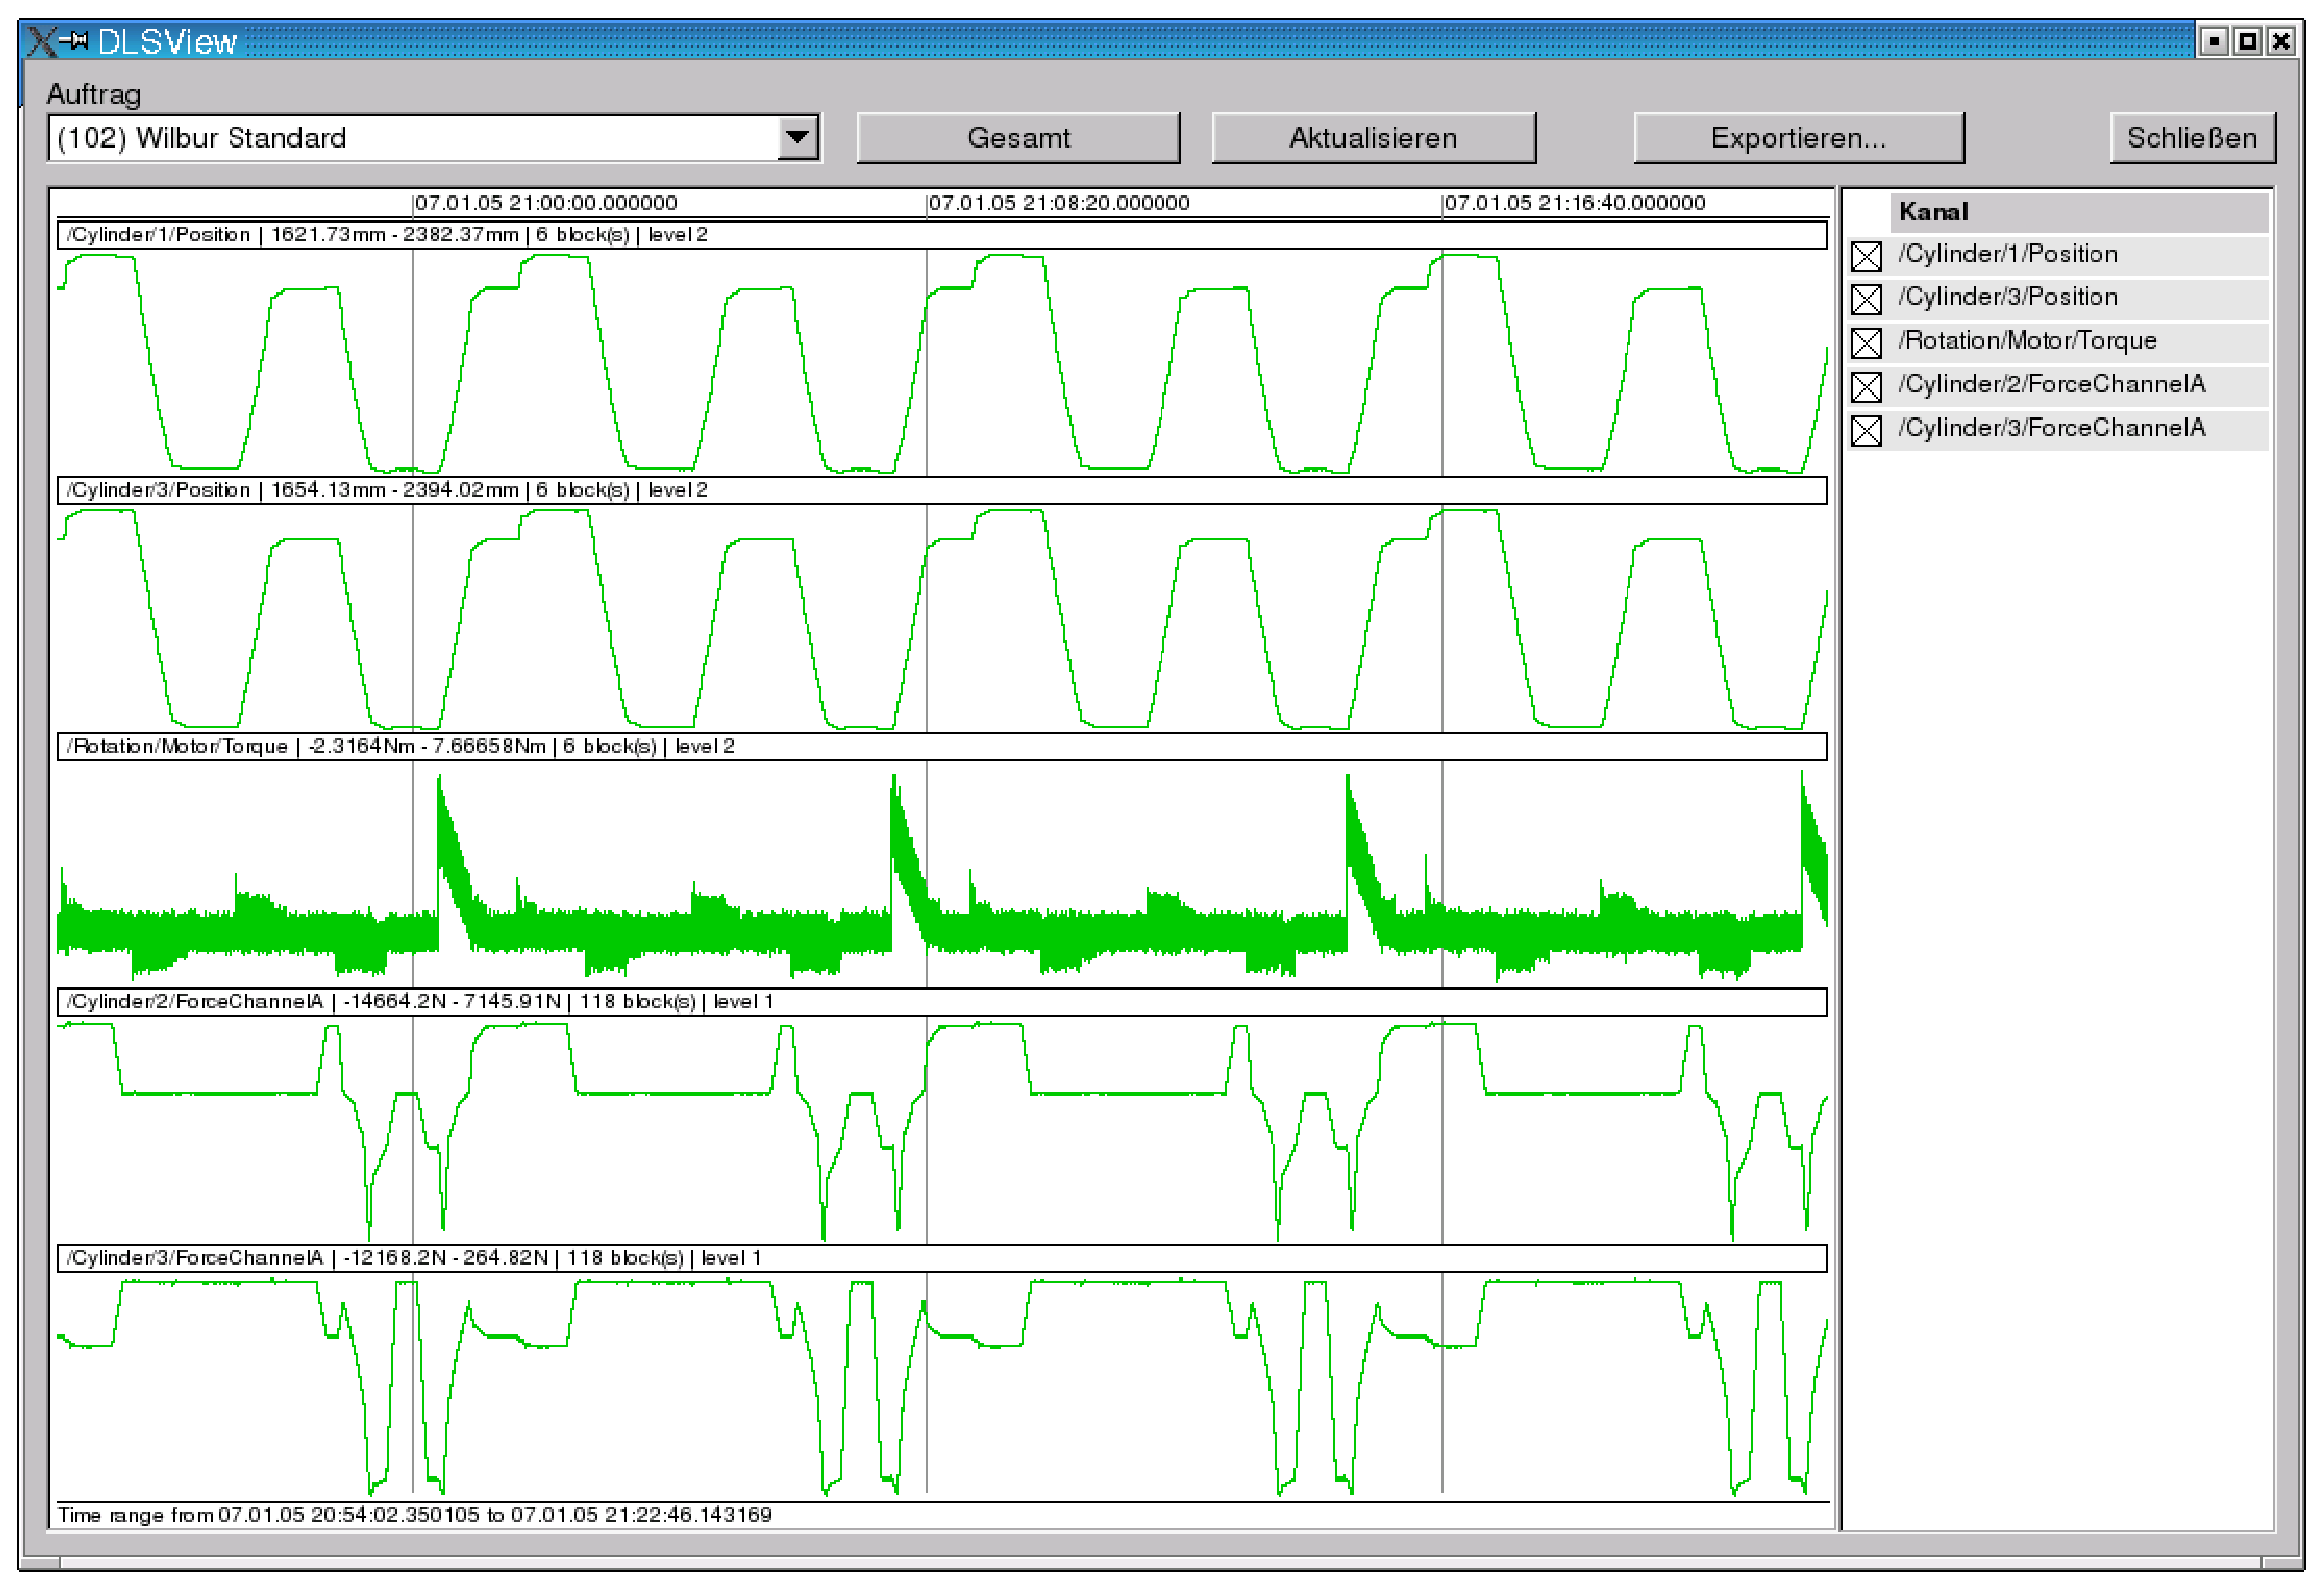
\includegraphics[width=\textwidth]{bilder/view_normal}
  \end{center}
  \caption{Fen\^etre principale de DLS View}
  \label{fig:dls_view_main}
\end{figure}

%------------------------------------------------------------------------------

\subsection{Description}

\begin{itemize}

\item Dans le coin sup\'erieur gauche de l'\'ecran, il y a un champ
  pour s\'electionner la t\^ache d'acquisition dont les donn\'ees doivent
  \^etre affich\'ees.

\item Sur le cot\'e droit est affich\'e la liste des canaux contenus
  dans la t\^ache qui a \'et\'e s\'electionn\'ee.

\item La majeure partie de la fen\^etre est utilis\'ee pour afficher
  les donn\'ees.  Son architecture permet d'afficher les donn\'ees de
  plusieurs canaux les uns au dessous des autres en partageant le
  m\^eme axe temporel, affich\'e en haut du graphique. Les graduations
  apparaissent sous la forme de ligne verticales grises dans un
  syst\`eme de coordonn\'ees.

\item L'intervalle de temps ainsi repr\'esent\'e est indiqu\'ee
  dans une petite ligne de texte tout en bas du graphique.

\item Un petit ent\^ete au dessus de chaque canal, contient le nom du
  canal, la plage des valeurs affich\'ees, le nombre de blocs de
  donn\'ees charg\'ees et le m\'eta niveau utilis\'e (voir
  \autoref{sec:dlsd_data_meta}).  Sous l'ent\^ete, les donn\'ees sont
  repr\'esent\'ees sous forme de courbes.  Une courbe blue indique que
  les donn\'ees affich\'ees sont des donn\'ees g\'en\'eriques
  (m\'eta-niveau 0), si un m\'eta-niveau sup\'erieur est utilis\'e,
  alors la courbe correspondante est verte.

\item Si aucune donn\'ee n'est disponible pour l'intervalle de temps
  \`a afficher, alors la rang\'ee du canal est affich\'e avec un fond
  jaune (voir \autoref{fig:dls_view_scan}).

\item Puisque toutes les canaux doivent partager la hauteur globale de
  l'affichage, la hauteur de chaque rang\'ee diminue avec le nombre
  de canaux \`a afficher. Si cette hauteur devient inf\'erieure \`a une
  valeur d\'efinie, une barre de d\'efilement appara\^it \`a droite.

\end{itemize}

%------------------------------------------------------------------------------

\subsection{Utilisation}

\begin{itemize}

\item Dans la liste de s\'election ``Job'', l'utilisateur peut choisir
  la t\^ache d'acquisition qu'il veut afficher. La liste des canaux acquis
  est alors mise \`a jour.

\item L'utilisateur peut afficher ou cacher les canaux individuels
  dans la zone d'affichage en cochant les cases situ\'ees devant
  leurs noms respectifs dans la liste des canaux.

\item Cliquer sur le bouton ``All'' d\'etermine et affiche l'intervalle
  de temps complet dans lequel les donn\'ees ont \'et\'e acquises
  pour les canaux selectionn\'es.

  Si des canaux sont ajout\'es ou supprim\'es imm\'ediatement apr\`es,
  le nouvel intervalle de temps est recalcul\'e \`a nouveau.
  Cependant, si l'utilisateur choisit un autre intervalle de temps \`a afficher
  ce dernier est constamment appliqu\'e m\^eme si des canaux sont ajout\'es
  ou supprim\'es.

\item Cliquer sur le bouton ``Update'' recharge et r\'eaffiche toutes
  les donn\'ees de l'intervalle de temps s\'electionn\'e.

\item Cliquer sur le bouton ``Export\ldots'' ouvre le dialogue d'exportation
  (voir \autoref{sec:view_export}).

\item En appuyant et tenant le bouton gauche de la souris dans la zone de
  donn\'ee de l'affichage, l'utilisateur peut s\'electionner un nouvel
  intervalle de temps qui sera indiqu\'e par deux lignes rouges verticales
  tant que le bouton de la souris est maintenu enfonc\'e.
  Les valeurs temporelles exactes sont indiqu\'ees sur le bord sup\'erieur
  du graphique. Lorsque le bouton gauche de la souris est rel\^ach\'e,
  le nouvel intervalle de temps est accept\'e et les donn\'ees correspondantes
  sont charg\'ees.

  De cette fa\c con, le rel\^achement du bouton de la souris peut \^etre
  en dehors de la zone d'affichage, ce qui permet d'\'etendre l\'eg\`erement
  l'intervalle de temps affich\'e.

\item De mani\`ere similaire, en appuyant et tenant le bouton droit de
  la souris dans la zone d'affichage, l'intervalle de temps pr\'esent\'e
  peut \^etre d\'eplac\'e. Lorsque le bouton de la souris est
  rel\^ach\'e, le nouvel intervalle de temps est accept\'e.

\item Un double clic dans la zone d'affichage \'etend d'un facteur
  deux l'intervalle de temps pr\'esent\'e. Au pr\'ealable, il est
  centr\'e autour du point temporel qui a \'et\'e cliqu\'e. Si la touche
  \textit{Shift} est maintenue enfonc\'ee pendant le double clic, un
  facteur 10 est utilis\'e pour l'extension.

\item Si la zone d'affichage des donn\'ees a le focus du clavier,
  l'appui sur la touche \textit{Ctrl} dessine une ligne verticale
  de balayage qui passe par le point temporel point\'e par la souris
  (voir \autoref{fig:dls_view_scan}).  Si cette ligne croise une
  courbe affich\'ee, la valeur de la donn\'ee au point d'intersection
  sera affich\'ee.

  Comme la ligne de balayage n'est pas infiniment \'etroite, il est
  possible que plusieurs valeurs de donn\'ees soient concern\'ees dans
  la zone couverte par celle-ci. Dans ce cas, la zone enti\`ere de
  valeur des valeurs qui sont pr\'esentes ``sous`` la ligne de
  balayage sera marqu'ee par deux lignes horizontales correspondant au
  minimum et maximum (voir le troisi\`eme canal dans
  \autoref{fig:dls_view_scan}).

\end{itemize}

\begin{figure}[tbh]
  \begin{center}
    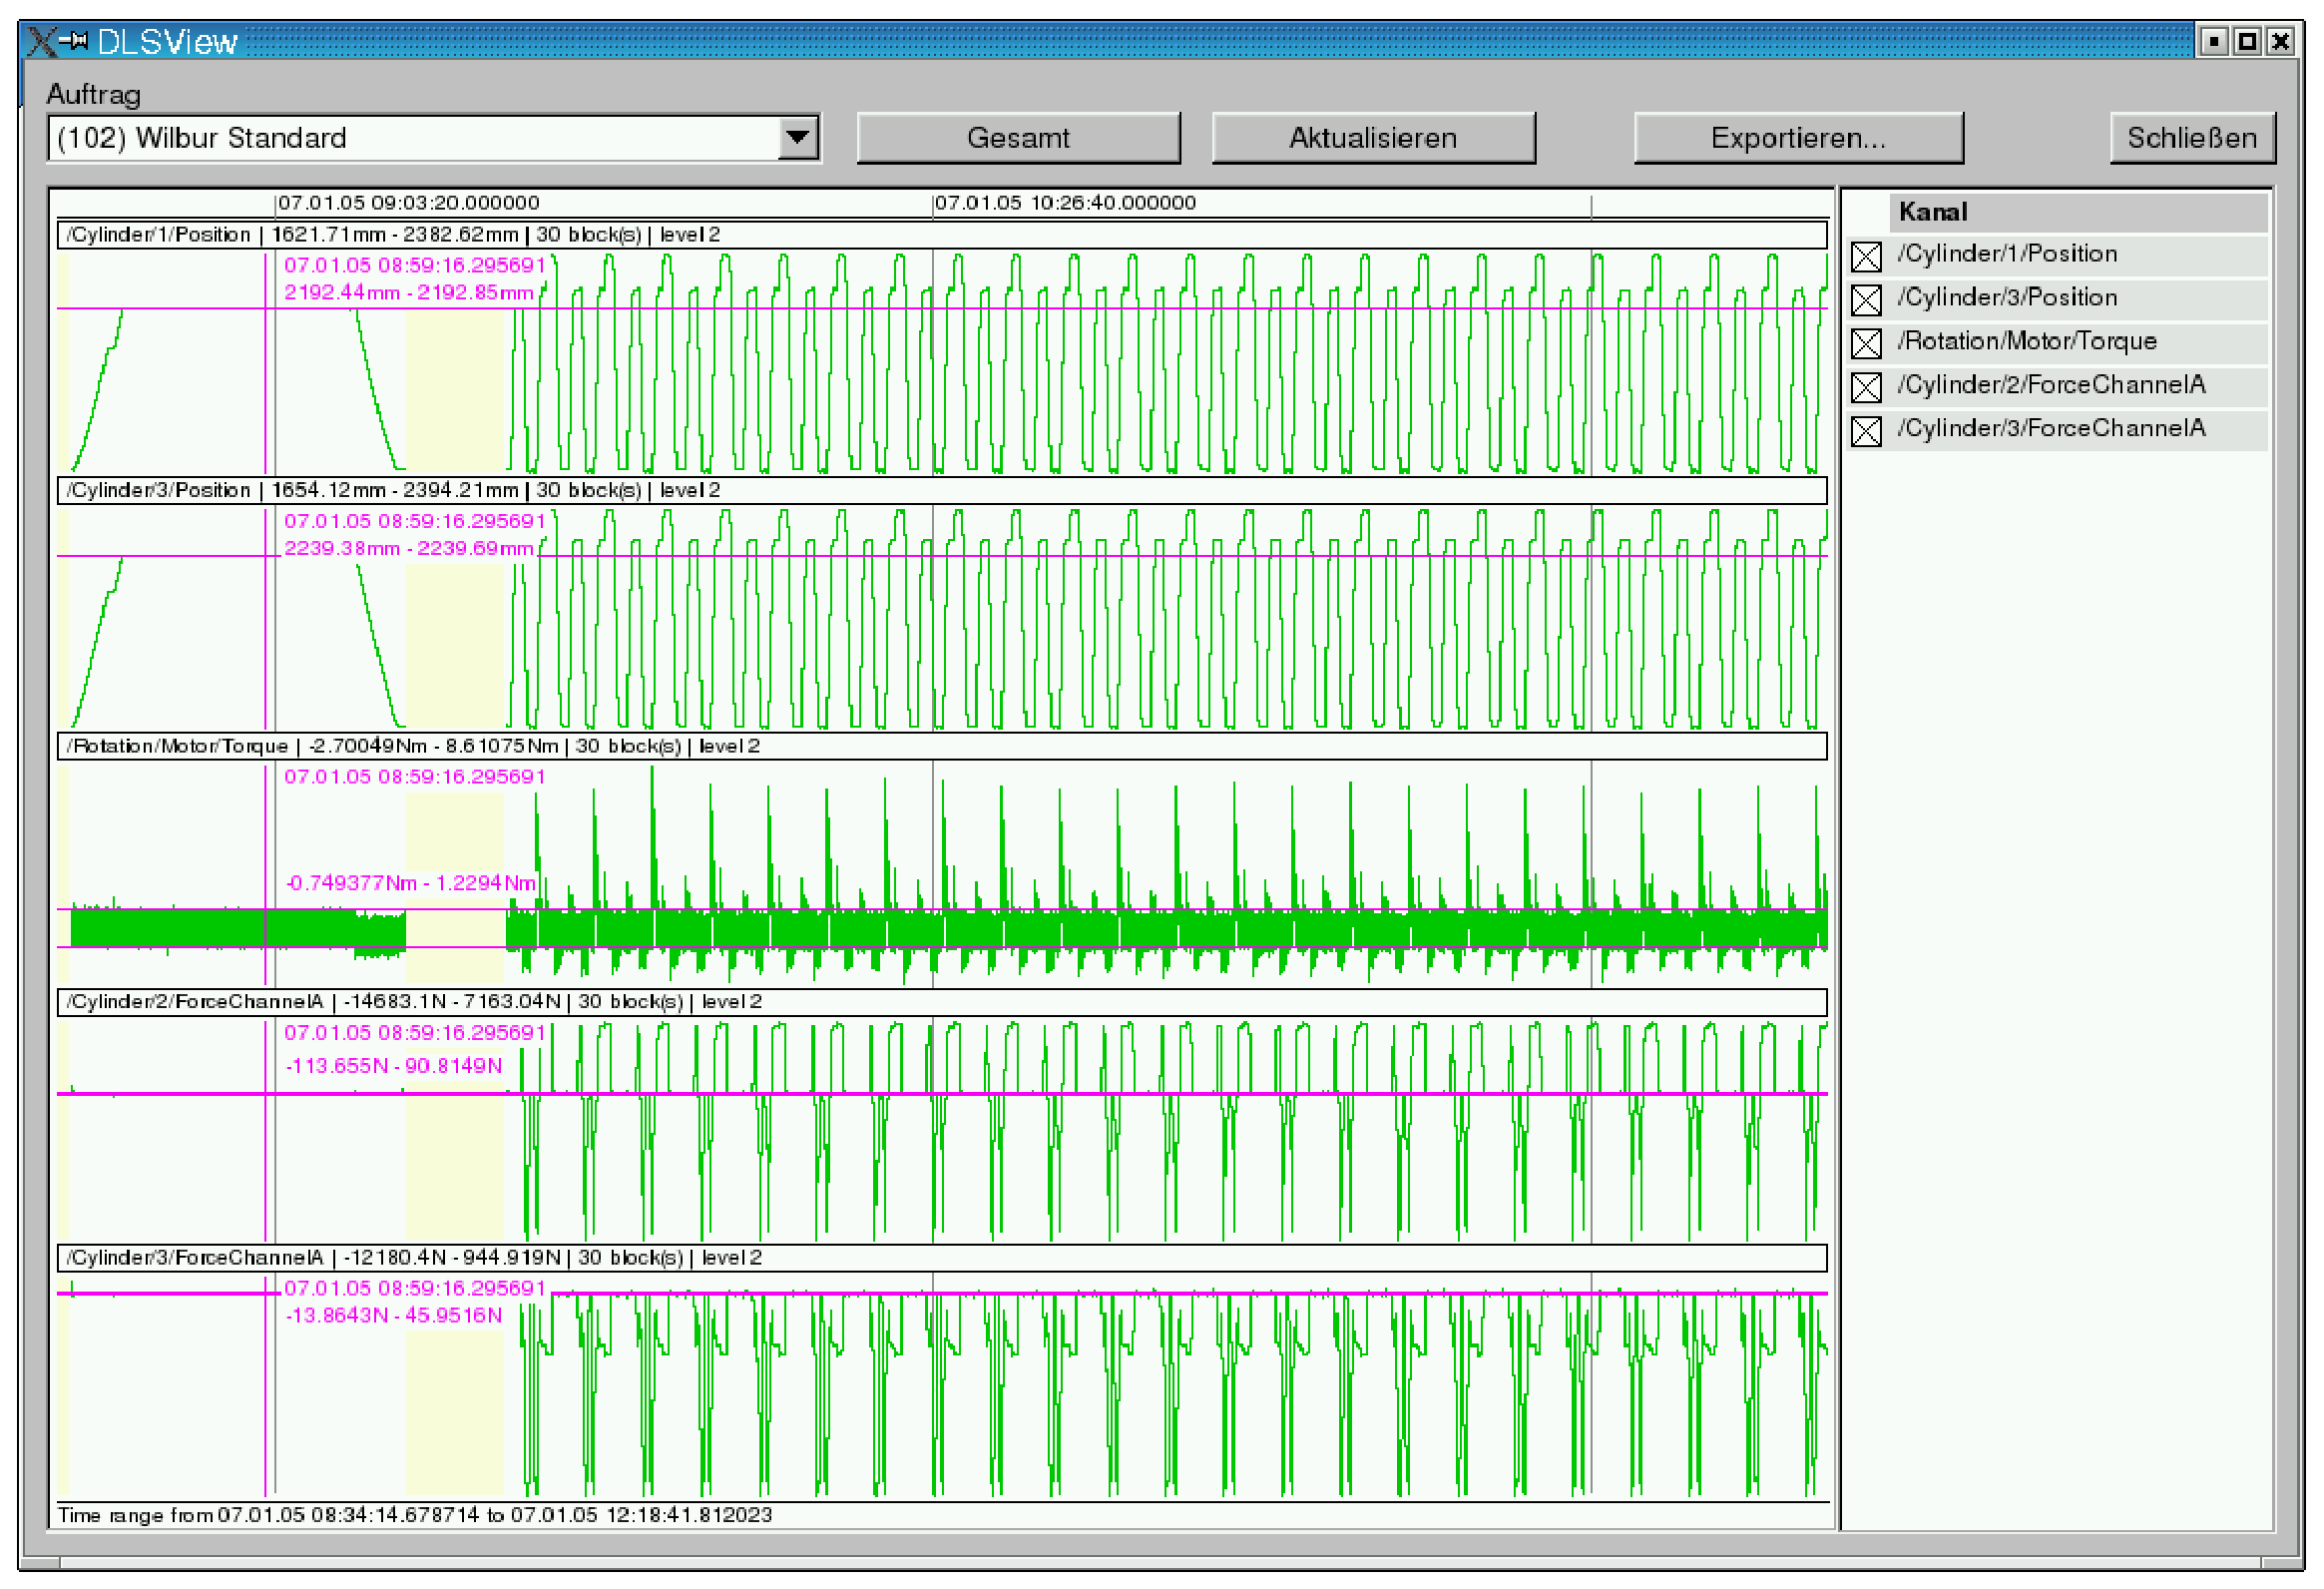
\includegraphics[width=\textwidth]{bilder/view_scan}
  \end{center}
  \caption{Ligne de balayage avec le bouton \textit{Ctrl} maintenu enfonc\'e}
  \label{fig:dls_view_scan}
\end{figure}

%------------------------------------------------------------------------------

\section{Le dialogue ``Export\ldots''}
\label{sec:view_export}

\begin{figure}[tbh]
  \begin{center}
    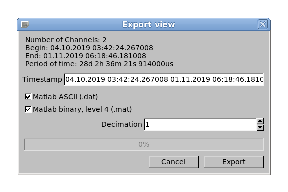
\includegraphics[width=.6\textwidth]{bilder/view_export_en}
  \end{center}
  \caption{Le dialogue d'exportation de DLS View}
  \label{fig:dls_view_export}
\end{figure}

%------------------------------------------------------------------------------

\subsection{Description}

\begin{itemize}

\item La partie sup\'erieure du dialogue (voir
  \autoref{fig:dls_view_export}) montre le nombre de canaux
  s\'electionn\'es et l'intervalle de temps choisi.
  L'exportation inclut toujours les donn\'ees
  affich\'ees dans la vue actuellement selectionn\'e dans la fen\^etre
  principale.

\item La barre de progression dans la partie inf\'erieure montrera par
  la suite la progression de l' exportation.

\end{itemize}

%------------------------------------------------------------------------------

\subsection{Utilisation}

\begin{itemize}

\item Dans la partie centrale du dialogue (voir \autoref{fig:dls_view_export})
  cocher les cases pour s\'electionner les formats d'exportation.

\item Un clic sur le bouton ``Export'' d\'emarre l'exportation des
  donn\'ees. Si la variable d'environnement
  \$DLS\_EXPORT\index{\$DLS\_EXPORT} est d\'efinie, les donn\'ees
  seront \'ecrites dans le r\'epertoire correspondant. Sinon, le
  r\'epertoire courant sera utilis\'e. Pour \'eviter d'\'ecraser des
  donn\'ees lors de l'exportation, un sous-r\'epertoire sera toujours
  cr\'e\'e pour accueillr les fichiers de donn\'ees.  Le nom de ce
  sous-r\'epertoire est d\'etermin\'e par la variable d'environnemnent
  \$DLS\_EXPORT\_FMT\index{\$DLS\_EXPORT\_FMT}, qui accepte les
  caract\`eres g\'en\'eriques conform\'ement aux conventions de la
  fonction c strftime().  Voir \texttt{man 3 strftime} pour la liste.
  Si la variable d'environnement n'a pas \'et\'e d\'efinie, le nom de
  r\'epertoire par d\'efaut
  \textit{dls-export-\%Y-\%m-\%d-\%H-\%M-\%S} est utilis\'e.


\item Le bouton ``Cancel'' interrompt l'exportation et ferme le dialogue.

\end{itemize}

%------------------------------------------------------------------------------

\chapter{M\'ethodes de compression}
\label{sec:comp} \index{Compression}

La compression des donn\'ees acquises re\c cues depuis les sources de
donn\'ees sert \`a r\'eduire l'espace de stockage requis dans le syst\`eme
de fichier. Il s'applique toujours par bloc (c'est-\`a-dire un certain
nombre de valeurs qui sont toujours compressées ensemble)
dont l'utilisateur peut ajuster la taille dans les sp\'ecifications du canal.
Une distinction fondamentale est faite entre la compression sans-perte
et celle avec perte.

Le syst\`eme DLS supporte diff\'erents algorithmes de compression.
Puisque la plupart des algorithmes produisent une sortie au format binaire,
elles seront converties en Base64 avant d'\^etre enregistr\'ees dans les
fichiers de donn\'ees.
Cependant, cela augmente l'espace de stockage d'un tiers, mais avec l'avantage
que les donn\'ees compress\'ees sont disponibles sous forme
de caract\`eres ``imprimables'' et par cons\'equent codables en XML.
C'est pourquoi, toutes les m\'ethodes de compression de DLS ont le suffixe
\textit{/Base64}.

Les m\'ethodes de compression suivantes sont support\'ees par DLS:

\begin{description}

\item[ZLib/Base64] Une m\'ethode de compression simple mais efficace
  offrant une compression sans pertes. Voir \autoref{sec:comp_zlib}.

\item[MDCT/ZLib/Base64] Une m\'ethode de compression am\'elior\'ee qui
  traite les donn\'ees par une transformation et une quantification,
  puis enfin les compresse.  Voir \autoref{sec:comp_mdct}.

\end{description}


%------------------------------------------------------------------------------

\section{Compression avec ZLib}
\label{sec:comp_zlib}

M\'ethode de compression: ZLib/Base64\\
Type de donn\'ees compressibles: toutes.

La biblioth\`eque ``ZLib''\index{ZLib} (\url{http://www.gzip.org/zlib})
fournit des fonctions pour la compression sans perte de donn\'ees.
Le processus d'acquisition dlsd utilise ces fonctions dans la m\'ethode
de compression ZLib/Base64.
Par ailleurs, l'algorithme ZLib est utilis\'e pour prendre en charge
d'autres processus ult\'erieurs pour compresser davantage les donn\'ees d\'ej\`a
trait\'ees.

Comme ZLib produit des sorties binaires, elles sont enregistr\'ees en Base64 pour tous les processus.

%------------------------------------------------------------------------------

\section{Compression avec MDCT}
\label{sec:comp_mdct} \index{MDCT}

M\'ethode de compression: MDCT/ZLib/Base64\\
Type de donn\'ees compressibles: \textit{TFLT} (float), \textit{TDBL} (double)

La m\'ethode de compression MDCT (``modified, discrete cosinus
transformation'') de DLS est un processus hybride
dans lequel les donn\'ees sont premi\`erement transform\'ees avec MDCT,
puis quantifi\'ees et finalement transpos\'ees par bit, dans
le but de rendre plus efficace leur compression avec ZLib.
Le but ici, est de compresser les donn\'ees acquises avec une erreur
limit\'ee.

\subsection{MDCT}

MDCT est une sorte d'\'equivalent discret de la transform\'ee
de Fourier qui transforme un signal dans son \'equivalent dans le domaine
fr\'equentiel qui \`a sont tour permet de retrouver le signal original.

Alors que la transformation ``normale'' DCT est fond\'e sur le
principe que $n$ valeurs sont transform\'ees en $n$ coefficients \`a
partir desquels le signal original peut \^etre compl\`etement
r\'ecup\'er\'e, la transformation ``modifi\'ee'' DCT transforme
toujours $n$ valeurs en $\frac{n}{2}$ coefficients qui forme une
repr\'esentation incompl\`ete du signal original.  Cependant, comme la
transformation est effectu\'ee avec un recouvrement de 50\%, le signal
original peut \^etre recup\'er\'e en re-chevauchant et re-transformant
deux s\'equences successives de coefficients.  Cette m\'ethode est
expliqu\'ee dans \autoref{fig:comp_mdct}.

\begin{figure}[htb]
  \begin{center}
    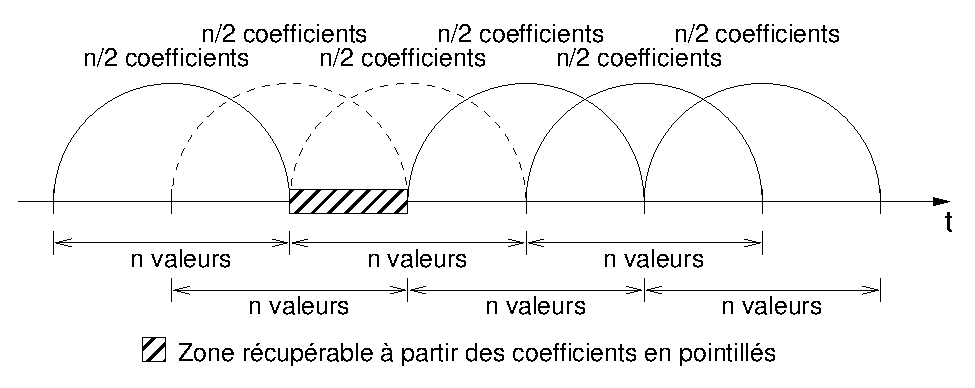
\includegraphics[width=300pt]{bilder/mdct_fr}
  \end{center} \caption{MDCT: Modified, discrete cosinus transformation}
  \label{fig:comp_mdct}
\end{figure}


Ce DCT modifi\'ee est compl\'et\'ee par le recouvrement des valeurs
\`a transformer au moyen d'une fonction fen\^etre qui donne un poids
plus faible aux valeurs \`a la marge.  Ceci emp\^eche que
diff\'erentes erreurs sur les zones marginales des transformations ne
conduisent \`a des ``artefacts'' afin que le signal original puisse
\^etre r\'ecup\'e de mani\`ere transparente.


\subsection{Quantification}

Les coefficients constat\'es par MDCT sont soumis \`a une
quantification enti\`ere. Ici une m\'ethode de bisection permet de
d\'ecider combien de bits au minimum la quantification doit conserver
pour \'eviter que l'erreur maximum commise ne devienne trop importante
lors de la transformation inverse. La m\'ethode de quantification
fournit non seulement des coefficients quantifi\'es sur $n$ bits mais
aussi le facteur d'\'echelle flottant requis pour r\'ecup\'erer les
coefficients originaux.

Comme l'erreur maximale commise ne peut pas \^etre d\'etermin\'ee avec
pr\'ecision pour une transformation MDCT inverse individuelle, elle
est estim\'ee comme la moiti\'e de l'erreur donn\'ee.  Quand deux
s\'equences de retransformations des coefficients sont superpos\'ees
pour r\'ecup\'erer le signal original, l'erreur donn\'ee ne peux
\^etre d\'epass\'ee aussi longtemps que l'erreur absolue dans les deux
signaux partiels ne d\'epasse pas la moiti\'e de l'erreur maximale
totale.

Les signaux des processus techniques sont souvent les plus adapt\'es
\`a une transformation par MDCT car, dans la plupart des cas, ils
r\'esultents de vibrations harmoniques superpos\'ees.  Cela signifie
que les portions hautes fr\'equences des coefficients pertinents sont
souvent peu prononc\'es et peuvent \^etre largement adapt\'es par la
quantification. Cela conduira ult\'erieurement \`a une bonne
compressibilit\'e.

\subsection{Transposition}
\label{sec:comp_mdct_trans}

La transposition est n\'ecessaire parce que la m\'ethode de
compression ZLib fonctionne par octet et dans la plupart des cas elle
ne parvient pas \`a reconna\^itre des mod\`eles de bits similaires.
Aussi, les bits individuels des coefficients quantifi\'es sont
retri\'es en m\'emoire.  Dans ce but, les coefficients sont
premi\`erement s\'epar\'es de leurs signes alg\'ebriques.  Les bits de
signes sont enregistr\'es s\'epar\'ement avant les bits des
coefficients.  Ils sont premi\`erement suivis par tous les
\textit{MSB}s (``Most Significant Bits'') (bits de poids forts) des
coefficients et enfin par tous les \textit{LSB}s (``Least Significant
Bits'') (bits de poids faibles).  En raison des coefficients
g\'en\'eralement tr\`es faibles des fr\'equences les plus \'elev\'ees,
un grand nombre d'octets sont \`a z\'ero et peuvent \^etre facilement
compress\'es.

Par cons\'equent, un bloc MDCT compress\'e se compose
du facteur d'\'echelle des coefficients quantifi\'es (4 ou 8 octets),
la quantit\'e $q$ de bits de quantification utilis\'es (1 octet),
de $n$ bits de signe et enfin de $q \cdot (n - 1) $ bits de coefficients.

\subsection{MDCT via FFT (Fast Fourier Transform)}

Marios Athineos\footnote{marios@ee.columbia.edu,
  \url{http://www.ee.columbia.edu/~marios}, Columbia University} a
d\'evelopp\'e une m\'ethode pour r\'eduire un MDCT portant sur $n$
valeurs \`a une transform\'ee de Fourier portant sur $\frac{n}{4}$
valeurs.  DLS utilise cette m\'ethode en combinaison avec la
biblioth\`eque \textit{FFTW3} (voir \autoref{sec:apx_install})
pour r\'eduire consid\'erablement la quantit\'e de calcul n\'ecessaire.
Cette biblioth\`eque combine des algorithmes efficaces pour le calcul
de la transform\'ee de Fourier avec l'utilisation des extentions processeurs
telles que MMX ou SSE.

%------------------------------------------------------------------------------

\section{Compression au travers de la quantification}
\label{sec:comp_quant} \index{quantisation}

M\'ethode de compression: Quant/ZLib/Base64\\
Types de donn\'ees compressibles: \textit{TFLT} (float), \textit{TDBL} (double)

Cette m\'ethode compression affaiblie soumet les valeurs de donn\'ees
\`a compresser \`a une quantification absolue, les diff\'erencie et
enfin les stocke sous forme transpos\'ee.  Cette m\'ethode pr\'epare les
``donn\'ees brutes'' afin que la compression ult\'erieure avec ZLib
soit encore plus efficace.

\subsection{Quantification}

Durant la quantification, les valeurs (en virgule flottante) sont
distribu\'ees via un facteur d'\'echelle sur un intervalle limit\'e
d'entiers naturels.  Une compression est obtenue en essayant de garder
cet intervalle aussi petit que possible afin de pouvoir coder les
valeurs quantifi\'ees avec quelques bits. Cependant, cela n'est fait
que si l'erreur produite reste sous une certaine limite sp\'ecifi\'ee
par l'utilisateur.

\subsection{Diff\'erentiation}

De plus, les valeurs quantifi\'ees sont diff\'erenci\'ees pour que les
formes d'onde du signal lin\'eaire deviennent plus harmonis\'ees dans
le codage afin que l'algorithme ZLib puisse mieux compresser les
donn\'ees.  \`A cette fin, au d\'ebut de l'ensemble de donn\'ees
compress\'es, le d\'ecalage (entier) est stock\'e, et \`a partir de
l\`a, seule la diff\'erence de valeur \`a valeur est stock\'ee.

\subsection{Transposition}

La transposition est faite pour les m\^eme raisons que pour
\textbf{MDCT/ZLib/Base64} method. Voir \autoref{sec:comp_mdct_trans}
\`a ce sujet.

%------------------------------------------------------------------------------

\appendix

\chapter{Installation de DLS}
\label{sec:apx_install} \index{Installation}

\section{Configuration requise}

DLS est principalement impl\'ement\'e avec le langage de programmation
C++\index{C++}. Pour sa compilation et son fonctionnement DLS a besoin
du syst\`eme d'exploitation Linux\index{Linux}.

Les logiciels suivants doivent \^etre install\'es pour la compilation
et l'ex\'ecution:

\begin{itemize}

\item \textit{syslogd}\index{syslogd}, qui fait habituellement partie
  de chaque distribution Linux, est utilis\'e pour enregistr\'e les
  messages \'emits pendant l'ex\'ecution.

\item Pour la compilation de l'interface graphique utilisateur de DLS
  Manager\index{DLS Manager} et DLS View\index{DLS View}, il est
  n\'ecessaire d'avoir la biblioth\`eque graphique
  \textit{FLTK}\index{FLTK} en version 1.1.  Celle ci peut \^etre
  t\'el\'echarg\'ee depuis le site web FLTK \url{http://www.fltk.org}.
  La biblioth\`eque doit \^etre compil\'ee avec le support pour le
  multithreading\footnote{Malheureusement, certaines distributions ne
    fournissent qu'un paquet sans multithreadind, dans ce cas la
    biblioth\`eque FLTK doit \^etre recompil\'ee.}  (option de
  configuration \texttt{--enable-threads}).

\item La biblioth\`eque \textit{ZLib} est requise pour la compression.
  Elle est incluse dans quasiment toutes les distributions Linux.
  En cas de besoin, elle peut \^etre t\'el\'echarg\'ee depuis
\url{http://www.gzip.org/zlib} et install\'ee.

\item La biblioth\`eque \textit{FFTW3} est aussi requise pour la
  compression.  Elle permet \`a DLS de calculer la transform\'ee de
  Fourier pour la compression MDCT. La biblioth\`eque peut \^etre
  t\'el\'echarg\'ee depuis \url{http://www.fftw.org/download.html}.

\item Pour DLS Manager et FLTK, vous aurez besoin de la biblioth\`eque
  \textit{pthreads}.

\end{itemize}

\section{Installation}

Apr\`es avoir copi\'e l'archive DLS depuis le CD
\textsuperscript{\textregistered} ou bien depuis le site
web EtherLab\textsuperscript{\textregistered}
\url{http://etherlab.org}, vous pouvez l'extraire:

\begin{lstlisting}
`\$` `\textbf{tar xjf dls-1.0-rXXX.tar.bz2}`
`\$` `\textbf{cd dls-1.0-rXXX.tar.bz2}`
\end{lstlisting}

Maintenant le code source peut \^etre configur\'e et
compil\'e avec les commande mentionn\'ees ci-dessous.
La commande \texttt{configure} reconna\^it les param\`etres
\texttt{--with-fltk-dir} et \texttt{--with-fftw3-dir} pour sp\'ecifier
le r\'epertoire d'installation des biblioth\`eques correspondantes.
Le r\'epertoire d'installation par d\'efaut de DLS est  \textit{/opt/etherlab}.
Un autre r\'epertoire d'installation peut \^etre sp\'ecifi\'e avec le
param\`etre \texttt{--prefix}.

\begin{lstlisting}
`\$` `\textbf{./configure}`
`\$` `\textbf{make}`
\end{lstlisting}

L'appel suivant (sous \textit{root}) installera tous les
ex\'ecutables, scripts et mod\`eles de fichiers de configurations
n\'ecessaires.

\begin{lstlisting}
# `\textbf{make install}`
\end{lstlisting}



\section{Configurer DLS en tant que service}

Si DLS doit \^etre configur\'e en tant que service, les scripts
\textit{init}, \textit{sysconfig} et \textit{profile} doivent \^etre
copi\'es dans les r\'epertoires appropri\'es de la distribution Linux.
Les commandes suivantes sont adapt\'ees pour la distribution Linux
SUSE mais seront l\'eg\`erement diff\'erentes pour d'autres
distributions:

\begin{lstlisting}
# `\textbf{cd /opt/etherlab}`
# `\textbf{cp etc/init.d/dls /etc/init.d/dls}`
# `\textbf{cp etc/sysconfig/dls /etc/sysconfig/dls}`
# `\textbf{cp etc/profile.d/dls /etc/profile.d/dls}`
# `\textbf{insserv dls}`
\end{lstlisting}

La configuration se fait en ajustant le fichier
\textit{/etc/sysconfig/dls}. Les variables de configurations
pertinentes sont document\'ees dans le fichier. Elles seront ensuite
export\'ees comme variables d'environnement par le script \textit{profile}
et mise \`a disposition de tous les utilisateurs.

Le r\'epertoire de donn\'ees DLS sera automatiquement cr\'e\'e au
d\'emarrage de DLS manager.  Pour cela, la variable d'environnement
\$DLS\_DIR\index{\$DLS\_DIR} doit \^etre d\'efinie ou bien le
r\'epertoire \`a utiliser doit \^etre sp\'ecifi\'e avec le param\^etre
\texttt{-d}.  Si le r\'epertoire indiqu\'e n'est pas encore un
r\'epetoire de donn\'ee DLS, le programme demande \`a l'utilisateur
s'il veut l'initialiser ainsi.

%------------------------------------------------------------------------------

\chapter{Type de donn\'ees}
\label{sec:apx_types}

\autoref{tab:typen} montre tous les types de donn\'ees support\'es pour les canaux\index{channel!data types} et les m\'ethodes de compressions possibles.

\begin{table}[htb]
  \centering
  \caption{Supported channel data types}
  \label{tab:typen} \vspace{1.5ex}
  \begin{tabular}[thb]{|l|l|l|}
    \hline
    \textbf{Type}   & \textbf{Description}         & \textbf{Compression}\\ \hline
    \textit{TCHAR}  & Entier 1 octet (avec signe)  & ZLib/Base64\\ \hline
    \textit{TUCHAR} & Entier 1 octet (sans signe)  & ZLib/Base64\\ \hline
    \textit{TINT}   & Entier 4 octets (avec signe) & ZLib/Base64\\ \hline
    \textit{TUINT}  & Entier 4 octets (sans signe) & ZLib/Base64\\ \hline
    \textit{TLINT}  & Entier 8 octets (avec signe) & ZLib/Base64\\ \hline
    \textit{TULINT} & Entier 8 octets (sans signe) & ZLib/Base64\\ \hline
    \textit{TFLT}   & Virgule flottante 4 octets & ZLib/Base64,\\
                    &                            & MDCT/ZLib/Base64,\\
                    &                            & Quant/ZLib/Base64\\ \hline
    \textit{TDBL}   & Virgule flottante 8 octets & ZLib/Base64,\\
                    &                            & MDCT/ZLib/Base64,\\
                    &                            & Quant/ZLib/Base64\\ \hline
  \end{tabular}
\end{table}

%------------------------------------------------------------------------------

\chapter{Fichiers PID} \label{sec:apx_pid}

\`A plusieurs endroits, le syst\`eme DLS utilise des fichiers
\textit{PID}\index{PID files}, un m\'ecanisme pour \'eviter que
plusieurs processus n'essayent d'ex\'ecuter une t\^ache unique.  Un
fichier \textit{PID} contient, sous forme \textit{ASCII}, le processus
ID (\textit{PID}) du processus en cours d'ex\'ecution.  Apr\`es le
d\'emarrage de chaque processus, celui-ci v\'erifie si le fichier PID
et le processus associ\'e PID existent.  Si les deux existent
d\'ej\`a, un nouveau processus ne doit pas \^etre d\'emarr\'e et donc
le nouveau processus doit s'arreter imm\'ediatement.  Si aucune autre
instance n'existe, le nouveau processus doit continuer son ex\'ecution
et cr\'eer un nouveau fichier PID. Avant cela, le fichier \textit{PID} obsol\`ete
(c'est-\`a-dire que le processus sp\'ecifi\'e n'existe plus) peut \^etre supprim\'e.

%------------------------------------------------------------------------------

\chapter{Param\`etre de ligne de commande}

%------------------------------------------------------------------------------

\section{dlsd}
\index{dlsd!Command line parameters}

\begin{lstlisting}
dlsd 1.4.0-rc2 revision de0a3e76b9ae
Usage: dlsd [OPTIONS]
  -d <dir>      Set DLS data directory.
  -u <user>     Switch to <user>.
  -n <number>   Set maximal number of open files.
  -k            Do not detach from console.
  -w <seconds>  Wait time before restarting logging
                  process after an error. Default is 30.
  -b            Do not bind to network socket.
  -p <port>     Listen port or service name. Default is 53584.
  -r            Read-only mode (no data logging).
  -h            Show this help.
\end{lstlisting}

%------------------------------------------------------------------------------

\section{Script d'initialisation}
\index{Init-Script!Command line parameters}

(Le chemin peut varier suivant les distributions Linux.)

\begin{lstlisting}
USAGE: /etc/init.d/dls {start|stop|restart|status}
\end{lstlisting}

%------------------------------------------------------------------------------

\section{dls\_status}
\index{dls\_status!Command line parameters}

\begin{lstlisting}
Call: dls_status [OPTIONS]
Options:
        -d [directory]     DLS data directory
        -h                 Show this help
\end{lstlisting}

%------------------------------------------------------------------------------

\section{dls\_ctl}
\label{sec:apx_cmd_dlsctl}
\index{DLS Manager!Command line parameters}

DLS Manager est d\'ecrit dans \autoref{sec:manager}.

\begin{lstlisting}
dls_ctl 1.4.0-rc2 revision de0a3e76b9ae
Call: dls_ctl [OPTIONS]
        -d [directory]     DLS data directory
        -u [user]          DLS user
        -h                 Show this help
\end{lstlisting}

%------------------------------------------------------------------------------

\section{dls\_view}
\index{DLS View!Command line parameters}

\begin{lstlisting}
dls_view 1.4.0-rc2 revision de0a3e76b9ae
Call: dls_view [OPTIONS]
        -d [directory]   DLS data directory
        -h               Show this help
\end{lstlisting}

%------------------------------------------------------------------------------

\section{dls}
\label{sec:apx_cmd_dls}
\index{dls (Tool)!Command line parameters}

\begin{lstlisting}
  Usage: dls COMMAND [OPTIONS]
  Commands:
      list - List available chunks.
    export - Export collected data.
      help - Print this help.
  Enter "dls COMMAND -h" for command-specific help.
\end{lstlisting}

%------------------------------------------------------------------------------

\subsection{dls list}

\begin{lstlisting}
  Usage: 1. dls list [OPTIONS]
         2. dls list -j JOB [OPTIONS]

  Description:
         1. Lists all available jobs.
         2. Lists chunks in the specified job.

  Options:
          -d DIR   Specify DLS data directory.
          -j JOB   Specify job ID.
          -h       Print this help.
\end{lstlisting}

%------------------------------------------------------------------------------

\subsection{dls export}

\begin{lstlisting}
dls 1.4.0-rc2 revision de0a3e76b9ae
Usage: dls export [OPTIONS]
Options:
   -d DIR         DLS data directory. Default: $DLS_DIR
   -o DIR         Output directory. Default: $DLS_EXPORT_DIR or "."
   -f NAMEFMT     Naming format for export directory.
                  See strftime(3).
                  Default: $DLS_EXPORT_FMT or "dls-export-%Y-%m-%d-%H-%M-%S"
   -a             Enable ASCII exporter
   -m             Enable MATLAB4 exporter
   -j ID          Job to export (MANDATORY)
   -c CHANNELS    Indices of channels to export (see below).
                  Default: All channels
   -p CHANNEL     Path of one channel to export (see
                  below). This option may appear
                  multiple times. Default: All channels.
   -s TIMESTAMP   Start time (see below). Default: Start of recording
   -e TIMESTAMP   End time (see below). Default: End of recording
   -n DECIMATION  Export every n'th value.
   -g             Export messages.
   -l LANGUAGE    2-character language code for messages.
   -q             Be quiet (no progress bar)
   -h             Print this help
CHANNELS is a comma-separated list of channel indices.
   Use the minus sign to specify ranges.
   Examples: "2,4,9", "1-20", "2,4,13-15,42".
CHANNEL is a signal name, optionally prefixed with
   'FILE:', where FILE is the name of the exported
   channel data file. If FILE is empty, or there is no
   colon found, files are named according to the channel
   indices.
TIMESTAMP is a broken-down time with microsecond resolution:
   YYYY[-MM[-DD[-HH[-MM[-SS[-UUUUUU]]]]]] or
   YYYY[-MM[-SS[ HH[:MM[:SS[.UUUUUU]]]]]].
   Examples: "2006-08", "2005-08-15 13:14:58.896366"
\end{lstlisting}

%------------------------------------------------------------------------------

\section{dls\_quota}
\label{sec:apx_cmd_quota}
\index{dls\_quota!Command line parameters}

\begin{lstlisting}
Call: dls_quota [OPTIONS]
        -d [directory]     DLS data directory
        -i [seconds]       Verification interval (0 = single check)
        -k                 Not a daemon
        -h                 Show this help
\end{lstlisting}

%------------------------------------------------------------------------------

\printindex

\end{document}

%------------------------------------------------------------------------------
